% --------------------------------------------------------------------------------------------------------
%%% SETUP SECTION
% --------------------------------------------------------------------------------------------------------


% First we declare the type of the document. 
% Depending on the type some factors may change.
% Here we also enter the size of the paper and many other parameters
\documentclass[a4paper,12pt,twoside]{article}

% a4paper – A4 paper size
% 12pt – default font size
% twoside – twoside paper format

% --------------------------------------------------------------------------------------------------------
%% IMPORT SECTION

% In LaTex we can also import packages like in any programming language
% Let's go through the most important ones.

\usepackage{graphicx}
\usepackage[english]{babel}
\usepackage[fixlanguage]{babelbib}
\usepackage[procnames]{listings}
\usepackage{listings}
\usepackage{xcolor}

\definecolor{codegreen}{rgb}{0,0.6,0}
\definecolor{codegray}{rgb}{0.5,0.5,0.5}
\definecolor{codepurple}{rgb}{0.58,0,0.82}
\definecolor{backcolour}{rgb}{0.95,0.95,0.92}

\lstdefinestyle{mystyle}{
    backgroundcolor=\color{backcolour},   
    commentstyle=\color{codegreen},
    keywordstyle=\color{magenta},
    numberstyle=\tiny\color{codegray},
    stringstyle=\color{codepurple},
    basicstyle=\ttfamily\footnotesize,
    breakatwhitespace=false,         
    breaklines=true,                 
    captionpos=b,                    
    keepspaces=true,                 
    numbers=left,                    
    numbersep=5pt,                  
    showspaces=false,                
    showstringspaces=false,
    showtabs=false,                  
    tabsize=2
}

\lstset{style=mystyle}
\usepackage{xcolor}
\usepackage{geometry}
\geometry{
    a4paper, 
    left=25mm,
	top=25mm,
	textwidth=16cm,
	textheight=23cm
}
\usepackage{siunitx} 
\usepackage{amsmath,amssymb}
\usepackage{datetime} 
\usepackage{color}
\usepackage{float}
\usepackage{mathptmx}
\usepackage{enumitem}
\usepackage[T1]{fontenc}
\usepackage[utf8]{inputenc}
\usepackage{lipsum}
\usepackage{setspace}
\setstretch{1.5}
\usepackage{hyperref} 
\usepackage{apacite}
\bibliographystyle{apacite}
\usepackage{circuitikz}
\usepackage{tikz}
\usetikzlibrary{arrows}
\usepackage{adjustbox}
% graphicx - adds additional graphical features to LaTeX
% babel - allows you to use special symbols from other languages
% listing – adds code spaces to LaTeX.
% xcolor – allows to work with colors in LaTeX. Works well with previous package
% geometry – a beginner-friendly package that allow you to work in a simple way with layout of everything (margins, headers, footnotes)
    % textwidth and texthight mean the size of the textarea
% siunix – for writing numbers with units 
% amsmath –  better mathematical formulas
% amssymb –  more math symbols
% datetime – date and time formatting
% color – a more basic version of xcolor.
% float – without it, tables position more or less random, with this an writing \begin{table}[H] the table appears right where it is defined!
% mathptmx – a package for adding Times Roman font in both text and math formulas
% enumitem – extensive customization of lists, including modifying labels, adjusting spacing, and changing the appearance of list items.
% fontenc – allows to select font encoding
    % T1 – refers to a 8-bit font encoding, more complex compared to a 7-bit one.
% inputenc - Unicode characters directly in your LaTeX source code. It is necessary when you need to use characters outside of the ASCII range. By specifying the input encoding as the one you enter in parameters, you ensure that all displayable characters in selected encoding are available for input.
    % utf8 - defines encoding
% lipsum – easy and quick way for creating lorem ipsum (dummy) text
% setspace - control the line spacing in your LaTeX document. It provides options and user-level commands to change the spacing between lines of text. The package is commonly used when you want to modify the line spacing for a specific section or for the entire document.
    % with setstretch we change the line spacing.
% hyperref - creating hyperlinks in LaTeX documents. Can be used for bookmarks and citations.
% apacite - formatting citations and references in APA (American Psychological Association) style.
    % The line \bibliographystyle{apacite} specifies the style to be used for the bibliography.
% circuitikz – creating circuit diagrams
% tikz – a powerful tool for creating schemes and diagrams in LaTeX.


%% END OF IMPORT SECTION 
% --------------------------------------------------------------------------------------------------------
%% ADDITIONAL INPUT

% We use input command when we want to import the content of another .tex file into the current one. So it is again very similar to the importing of local files in python.
% At this part it is also good to "import" some extra formatting and define your custom commands. For convenience and cleanliness of our code we are going to do it in separate files.

%% DEFINE CUSTOM COMMANDS AND SHORTCUTS

% some commands
\def\ba#1\ea{\begin{align}#1\end{align}}
\def\bas#1\eas{\begin{align*}#1\end{align*}}
\def\bmat#1\emat{\begin{pmatrix}#1\end{pmatrix}}
\newcommand{\ve}[1]{\vec{#1}}
\newcommand{\veTwo}[2]{\begin{pmatrix}#1\\#2\end{pmatrix}}
\newcommand{\veThree}[3]{\begin{pmatrix}#1\\#2\\#3\end{pmatrix}}
\newcommand{\veFour}[4]{\begin{pmatrix}#1\\#2\\#3\\#4\end{pmatrix}}
\newcommand{\ora}[1]{\overrightarrow{#1}}
\newcommand{\ola}[1]{\overleftarrow{#1}}
\newcommand{\s}[1]{\sqrt{#1}}

\def \bit{\begin{itemize}\setlength\itemsep{0em}} %\vspace{-5mm}
	\def \eit{\end{itemize}}

\def \ben{\begin{enumerate}\setlength\itemsep{0em}} %\vspace{-5mm}
	\def \een{\end{enumerate}}

\def \N{\mathbb{N}}
\def \Z{\mathbb{Z}}
\def \Q{\mathbb{Q}}
\def \R{\mathbb{R}}
\def \C{\mathbb{C}}

\def \ra{\rightarrow}
\def \longra{\longrightarrow}
\def \Ra{\Rightarrow}
\def \Longra{\Longrightarrow}
\def \la{\leftarrow}
\def \longla{\longleftarrow}
\def \La{\Leftarrow}
\def \Longla{\Longleftarrow}

\def \lra{\leftrightarrow}
\def \longlra{\longleftrightarrow}
\def \Lra{\Leftrightarrow}
\def \Longlra{\Longleftrightarrow}

\def \l{\left}
\def \r{\right}

\def \a{\alpha}
\def \b{\beta}
\def \g{\gamma}

\def \c{\cdot}

\def \el{\in}
\def \notel{\notin}

\newcommand{\f}{\frac}

\def \q{\quad}
\newcommand{\p}{\phantom}

\def\bs#1\es{\begin{split}#1\end{split}}


\def \L{\mathbb{L}}



%!TEX root = ../maturaarbeit.tex

%%%%%%%%%%%%%%%%%%%%%%%%%%%%%%%%%%
% DEFINE COLORS
\definecolor{red}{rgb}{0.6,0,0} 
\definecolor{blue}{rgb}{0,0,0.6}
\definecolor{green}{rgb}{0,0.8,0}
\definecolor{cyan}{rgb}{0.0,0.6,0.6}

\definecolor{mypink}{rgb}{0.753,0.000,0.890}
\definecolor{myblue}{rgb}{0.078,0.000,1.000}
\definecolor{mybluedark}{rgb}{0.004,0.024,0.525} \definecolor{mygreen}{rgb}{0.000,0.514,0.000}
\definecolor{myreddark}{rgb}{0.698,0.000,0.008}
\definecolor{mycyan}{rgb}{0.000,0.506,0.612}
\definecolor{mybrown}{rgb}{0.494,0.365,0.090}

%%% DISPLAY CODE
\usepackage{listings}
\newcommand\pythonstyle{\lstset{
    language=Python,
	tabsize=4,
	basicstyle=\normalsize\sffamily,
	numberstyle=\color{gray},
	stringstyle=\color{myreddark},
    commentstyle=\color{mygreen},
    % KEYWORDS
    % main keywords
	keywordstyle=\normalsize\color{myblue},%\bfseries,
    % add keywords (main blue)
    emph={False,None,True,self,TODO},
    emphstyle={\color{myblue}},
    % pink emph
    emph={[2]assert,break,continue,del,elif ,else,except,finally,for,from,global,if,import,in,pass,raise,return,try,while,with,yield},
    emphstyle={[2]\color{mypink}},%\bfseries,
    %dark blue emph
    emph={[3]execfile,reduce,xrange},
    emphstyle={[3]\color{mybluedark}},
    % brown emph
    emph={[4]exec,print,isinstance,zip,enumerate,reversed,len,repr},
    emphstyle={[4]\color{mybrown}},
    % cyan emph
    emph={[5]object,type,list,set,dict,tuple,str,super},
    emphstyle={[5]\color{mycyan}},
    % errors (also cyan emph)
    emph={[6]Exception,NameError,IndexError,SyntaxError,TypeError,ValueError,OverflowError,ZeroDivisionError},
    emphstyle={[6]\color{mycyan}},
    % errors (also cyan emph)
    emph={[7]copy,deepcopy,append,real,imag},
    emphstyle={[7]\color{black}},
    % 
    showstringspaces=false,
	breaklines=true,
	numbers=left,
    frame=tb,
	xleftmargin=15pt
}}

\newcommand\javascriptstyle{\lstset{
	basicstyle=\small\sffamily,
    keywordstyle=\color{blue}\bfseries,
    commentstyle=\color{purple}\ttfamily,
    stringstyle=\color{red}\ttfamily,
	numberstyle=\color{gray},
    keywords={typeof, new, true, false, catch, function, return, null, catch, switch, var, if, in, while, do, else, case, break},
    ndkeywords={class, export, boolean, throw, implements, import, this},
    ndkeywordstyle=\color{darkgray}\bfseries,
    identifierstyle=\color{black},
    comment=[l]{//},
    morecomment=[s]{/*}{*/},
    morestring=[b]',
    morestring=[b]",
    showstringspaces=false,
	breaklines=true,
	numbers=left,
    frame=tb,
	xleftmargin=15pt,
    sensitive=false,
}}

\newcommand\csharpstyle{\lstset{
	language=csh,
	tabsize=4,
	basicstyle=\small\sffamily,
	numberstyle=\color{gray},
	stringstyle=\color{myreddark},
    commentstyle=\color{mygreen},
	morecomment=[l]{//}, %use comment-line-style!
	morecomment=[s]{/*}{*/}, %for multiline comments
    % KEYWORDS
	keywordstyle=\normalsize\color{myblue},%\bfseries,
	morekeywords={ abstract, event, new, struct,
		as, explicit, null, switch,
		base, extern, object, this,
		bool, false, operator, throw,
		break, finally, out, true,
		byte, fixed, override, try,
		case, float, params, typeof,
		catch, for, private, uint,
		char, foreach, protected, ulong,
		checked, goto, public, unchecked,
		class, if, readonly, unsafe,
		const, implicit, ref, ushort,
		continue, in, return, using,
		decimal, int, sbyte, virtual,
		default, interface, sealed, volatile,
		delegate, internal, short, void,
		do, is, sizeof, while,
		double, lock, stackalloc,
		else, long, static,
		enum, namespace, string},
	% 
    showstringspaces=false,
	breaklines=true,
	numbers=left,
    frame=tb,
	xleftmargin=15pt	
}}

% Python environment
\lstnewenvironment{python}[1][]
{
	\pythonstyle
	\lstset{#1}
}
{}
\lstnewenvironment{javascript}[1][]
{
	\javascriptstyle
	\lstset{#1}
}
{}
\lstnewenvironment{csharp}[1][]
{
	\csharpstyle
	\lstset{#1}
}
{}

% CODE FOR EXTERNAL FILES
\newcommand\pythonexternal[2][]{{
		\pythonstyle
		\lstinputlisting[#1]{#2}}}

% CODE FOR INLINE
\newcommand\pythoninline[1]{{\pythonstyle\lstinline!#1!}}
\newcommand\csharpinline[1]{{\csharpstyle\lstinline!#1!}}
\newcommand\javascriptinline[1]{{\javascriptstyle\lstinline!#1!}}


%% END OF ADDITIONAL INPUT
% --------------------------------------------------------------------------------------------------------
%%% END OF SETUP SECTION 
% --------------------------------------------------------------------------------------------------------


% --------------------------------------------------------------------------------------------------------
%%% ACTUAL DOCUMENT 
% --------------------------------------------------------------------------------------------------------


% The next part is the body of the document
\begin{document}
    % Before we start adding anything it would be a good idea to define the language of the document

    \selectlanguage{english} % or german

    % Now we input our title page
    \begin{titlepage}
    % First we create an empty page
    \clearpage\thispagestyle{empty}
    \setstretch{1}

    % So here we are creating a kind of a header section (align to the top of the page ) which consists of two another sections which both take 50% (0,5) of the mother section: 
    \begin{minipage}[t]{\textwidth}
        \begin{minipage}[t]{0.5\textwidth}
            Andrii Zhabrovets\\
            Friedrichshafnerstrasse 54a\\
            8590 Romanshorn\\
            076 525 13 74\\
            anzhabro@ksr.ch
        \end{minipage}
        \begin{minipage}[t]{0.5\textwidth}
            \begin{flushright}
                Kantonsschule Romanshorn\\
                Klasse 3Mez\\
                SLA
            \end{flushright}
        \end{minipage}
    \end{minipage}

    % Now we make some vertical space
    \vspace{4cm}


    % We separate the next part of the code so that the title formatting applies only to the selected section
    {
    % Center our title in the middle
    \centering

    % Add title (huge size, bold) and \par is just to start new paragraph
    \Huge\bfseries Was ist die AR-Technologie (Augmented Reality) und welche Anwendungen gibt es in der realen Welt?\par

    \vspace{1cm}

    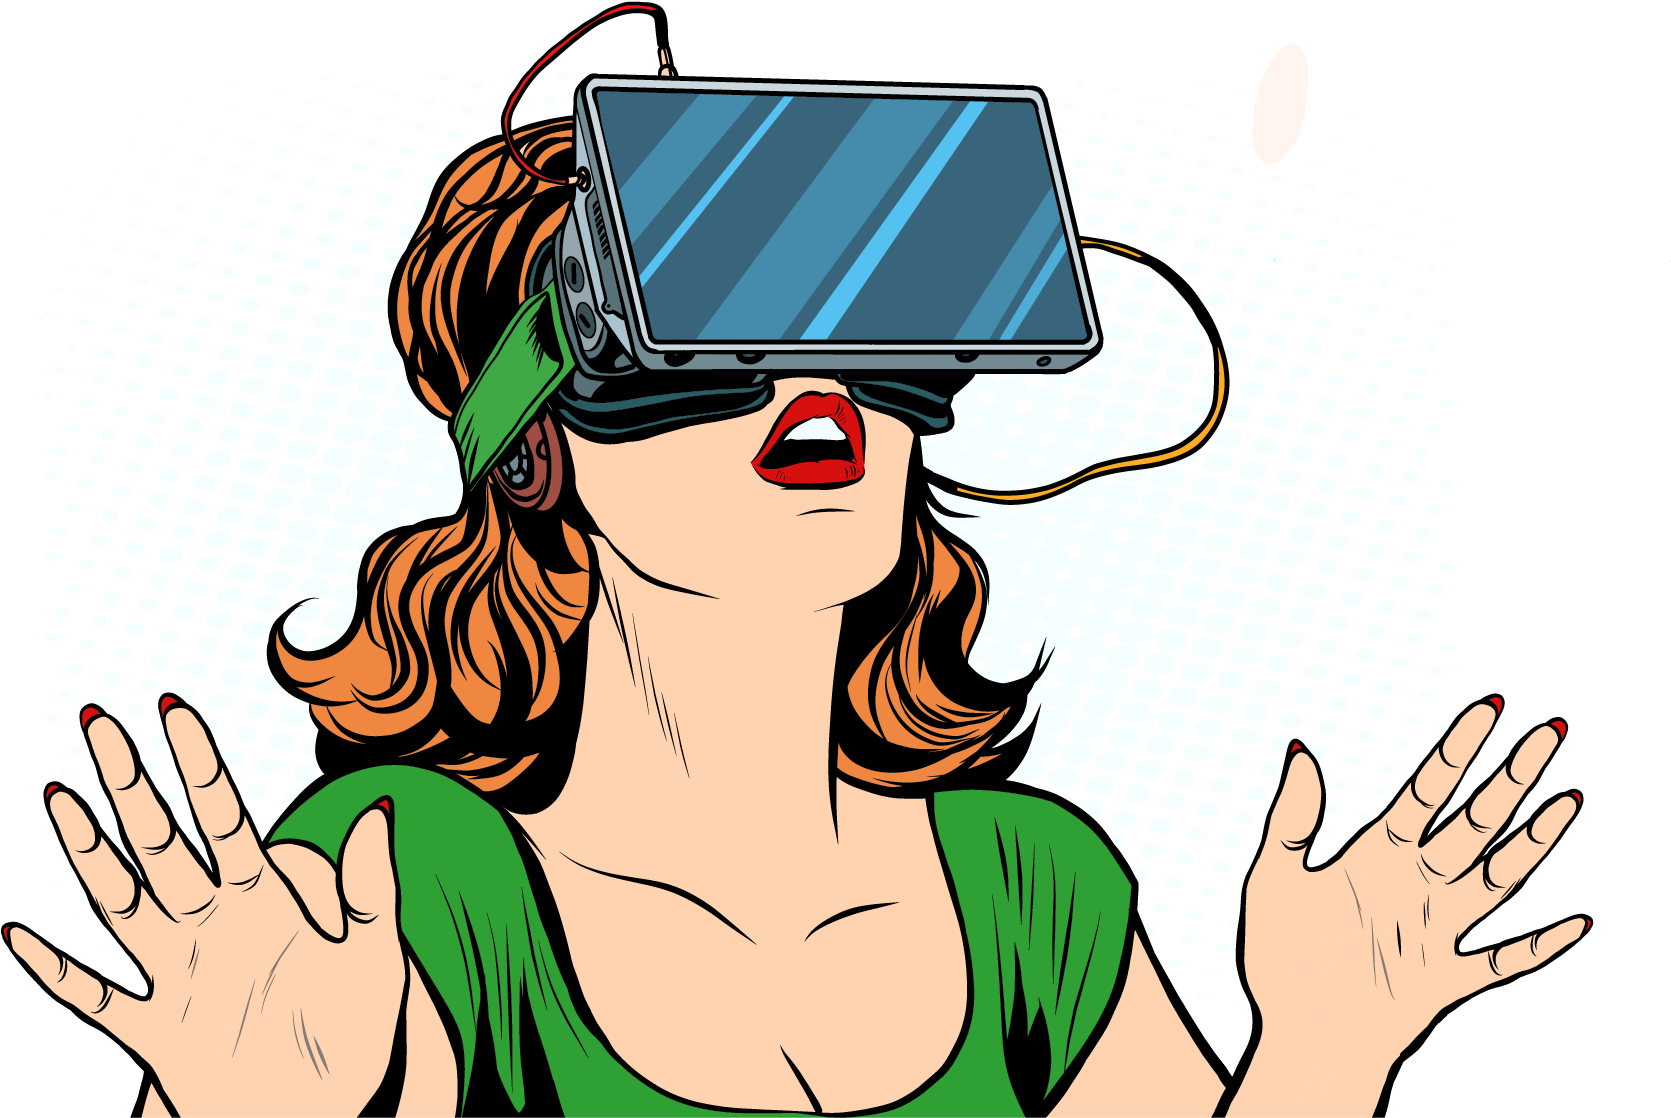
\includegraphics[width=0.5\textwidth]{attachments/ar.png}\par
    }

    % Now let's add a footer.
    \vspace{46mm}

    % No indent is similar to strip() in python
    \noindent
    Fach: Informatik\noindent \\ 
    Betreuungsperson: Dr. Andreas Schärer \\
    Abgabetermin: 11 September 2023 \\

\end{titlepage}


    % Page Numbering type. For abstract and table of contents we use roman numbers.
    \pagenumbering{roman}

    
\section*{Abstract}

% Die Technologie der Augmented Reality (Erweiterte Realität, AR), die digitale und physische Welten nahtlos miteinander verbindet, hat in den letzten Jahren zunehmend an Bedeutung gewonnen. Diese Arbeit untersucht die AR-Technologie aus theoretischer und technologischer Sicht und zeichnet ihre Entwicklung seit ihren Anfängen nach.  Die Arbeit untersucht gründlich die Vor- und Nachteile von aktuellen und möglichen Anwendungen von Augmented Reality in verschiedenen Bereichen wie Archäologie, Bildung, Medizin, Militär, Videospielen, Navigation und Übersetzung.
\textbf{To Be Done}



    \newpage
    \tableofcontents

    \parindent=0pt
    \parskip=6pt

    \newpage

    \pagenumbering{arabic}

    \section{Introduction}

The rapid advancements in Artificial Intelligence (AI) have brought transformative changes to numerous industries, with software engineering being a significant focus. AI-driven systems have moved beyond automation of routine tasks and now exhibit the potential to tackle complex challenges, including programming problem-solving. These developments have prompted critical discussions about whether AI can assume roles traditionally held by software engineers. Understanding the capabilities and limitations of these systems is essential for gauging their potential impact on the software development process.

This study explores the problem-solving capabilities of state-of-the-art AI models by evaluating their performance on programming tasks. Using a rigorous benchmarking framework, we assess these models through a set of common problems sourced from Leetcode, a platform widely acknowledged for its relevance in evaluating programming proficiency. By providing consistent prompts and analyzing their outputs, the research seeks to measure the effectiveness of AI in solving tasks of varying complexity and to draw meaningful comparisons with human performance.

The investigation centers on analyzing the technical skills of AI in problem-solving, identifying strengths and weaknesses, and determining its readiness to operate independently or alongside human developers. In doing so, this study also examines broader questions about the evolving role of AI in software engineering and its implications for the future of the profession.

The paper is structured to provide a comprehensive analysis of the topic, beginning with a review of existing literature to situate the research within the broader context of AI applications in software development. A detailed methodology follows, outlining the design and implementation of the benchmarks used for evaluating AI performance. The results are presented and analyzed to highlight key patterns and insights, culminating in a discussion of their implications for software engineering and AI research. Finally, the study concludes by reflecting on the findings and their relevance to the question of whether AI is capable of substituting software engineers.

By addressing these themes, this research aims to contribute to a deeper understanding of the capabilities of AI in software development and to inform future directions for improving AI systems in this domain.


    \newpage


    % \section{Augmented Reality}


\subsection {Definition}

Was ist AR?
Das Konzept der erweiterten Realität (Augmented Reality, AR) wurde von vielen Forschern der Informatik unter Berücksichtigung verschiedener Faktoren unterschiedlich definiert.

Die ersten Definitionen wurden von Milgram, Takemura, Utsumi und Kishino vorgeschlagen
(1994). In ihrer Arbeit “Augmented Reality: A class of displays on the reality-virtuality continuum” (Eine Klasse von Displays auf dem Realitäts-Virtualitäts-Kontinuum) konzeptualisierten sie das Virtual-Reality-Kontinuum, das vier Systeme berücksichtigt: reale Umgebung (Real Environment), erweiterte Realität (Augmented Reality), erweiterte Virtualität (Augmented Virtuality) und virtuelle Umgebung (Virtual Environment). Darüber hinaus wurden zwei Ansätze zur Definition von “Augmented Reality” genannt: eine breite Definition und eine präzisere Definition. In der breiten Definition wird Augmented Reality definiert als “Erweiterung des natürlichen Feedbacks an den Operator mit simulierten Hinweisen”. Im Gegensatz dazu wird sie im genaueren Verständnis definiert als “eine Form der virtuellen Realität, bei der das am Kopf montierte Display des Teilnehmers transparent ist und eine klare Sicht auf die reale Welt ermöglicht”.  \cite{Milgram94a} \cite{Milgram94b}
\vspace{1cm}
\begin{figure}[h!]
    \centering
    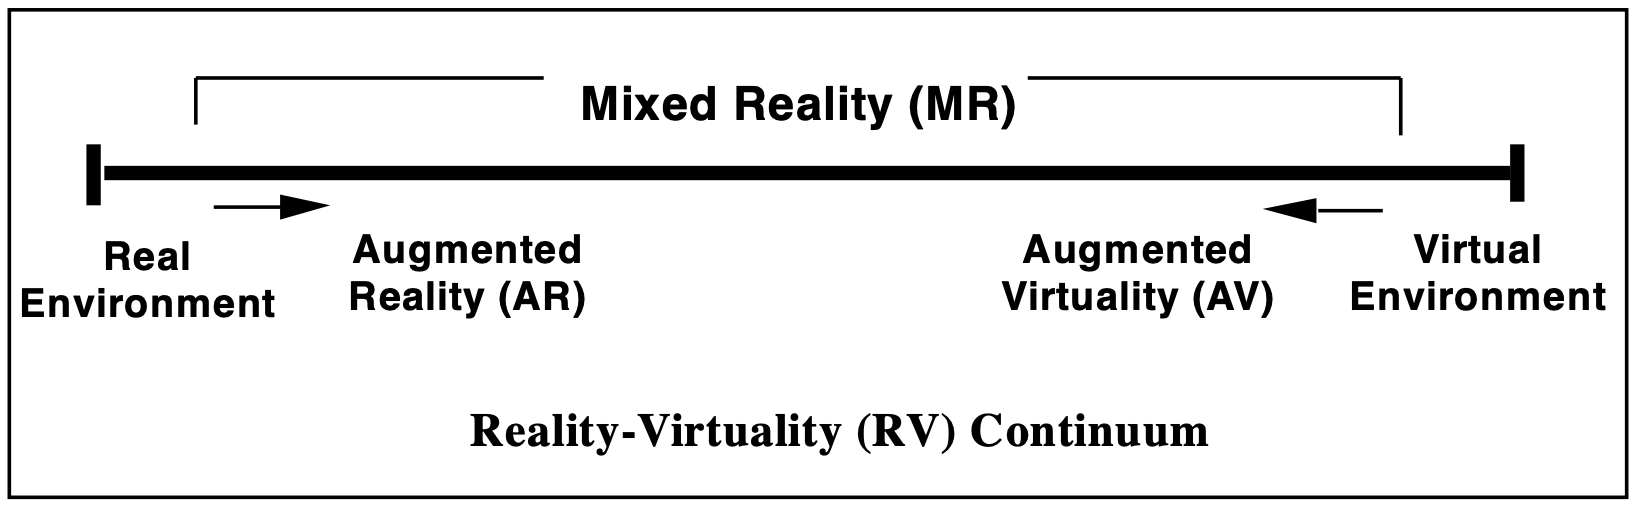
\includegraphics[width=0.9\textwidth]{attachments/MR_Definition.png}
    \caption{Vereinfachte Darstellung eines “Reality-Virtuality (RV) Continuum”.}  \cite{Milgram94a}
    \end{figure}
    

    \newpage

Andere Forscher, wie z. B. T. Azuma, definieren AR anhand seiner Merkmale oder Eigenschaften. Nach seinem Ansatz wird AR als Systeme definiert, die die folgenden drei Merkmale aufweisen:
\begin{enumerate}
    \item kombiniert reale und virtuelle Objekte in einer realen Umgebung;
    \item läuft interaktiv und in Echtzeit;
    \item registriert (richtet aus) in 3-D reale und virtuelle Objekte miteinander.  \cite{Azuma1997ASO}
\end{enumerate}


\subsection {Schlüsseltechnologien}

% An Augmented Reality System can be divided into two components: one is hardware, and the other is software  \cite{craig2013understanding}, \cite{Chatzopoulos}.
Ein Augmented-Reality-System kann in zwei Komponenten unterteilt werden: die Hardware und die Software \cite{craig2013understanding}, \cite{Chatzopoulos}.

% The main characteristic of the hardware components is to acquire and display the data and information, and process it. The \textbf{input components} are sensors that respond to physical or chemical stimuli from the real environment and provide the necessary data for the development of the system. The \textbf{output components} are devices for displaying the information, which can be divided into wearable and non-wearable, as well as optical, video, and projection devices. The output itself can be further divided into two variants of displays: \textbf{Optical See-through Display}, where the virtual contents are projected onto the interface to mix with the real scene optically, and \textbf{Video See-through Display}, which has two work modalities: one uses HMD (Head-Mounted Display) devices, and the other works with camera and screen in handheld devices, such as smartphones and tablets \cite{Azuma1997ASO}. 
Das Hauptmerkmal der Hardwarekomponenten ist die Erfassung und Anzeige der Daten und Informationen sowie deren Verarbeitung. Die \textbf{Input-Komponenten} sind Sensoren, die auf physikalische oder chemische Reize aus der realen Umgebung reagieren und die notwendigen Daten für die Entwicklung des Systems liefern. Die \textbf{Output-Komponenten} sind Geräte zur Anzeige der Informationen, die in tragbare und nicht tragbare sowie optische, Video- und Projektionsgeräte unterteilt werden können. Die Ausgabe selbst kann weiter in zwei Varianten von Displays unterteilt werden: \textbf{Optisch durchsichtiges Display (Optical See-through Display)}, bei dem die virtuellen Inhalte auf die Schnittstelle projiziert werden, um sich optisch mit der realen Szene zu vermischen, und \textbf{Video-Durchsichtiges Display (Video See-through Display)}, bei dem es zwei Arbeitsmodalitäten gibt: eine verwendet HMD-Geräte (Head-Mounted Display), die andere arbeitet mit Kamera und Bildschirm in Handheld-Geräten wie Smartphones und Tablets \cite{Azuma1997ASO}.

\newpage

\vspace{1cm}

\begin{figure}[h!]
    \centering
    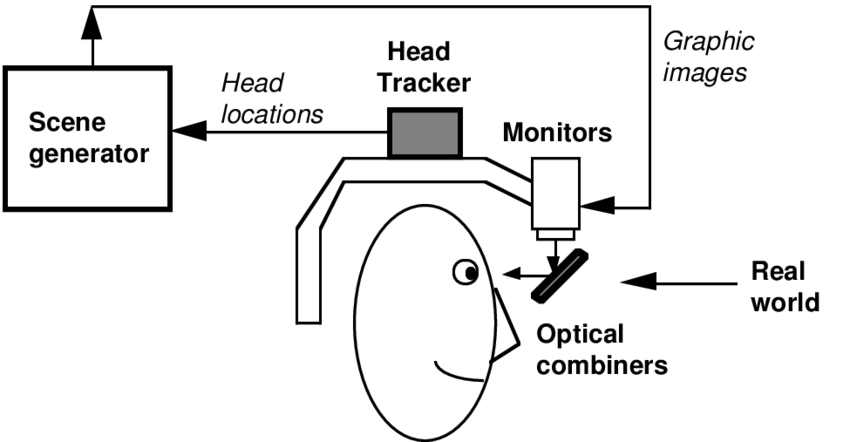
\includegraphics[width=0.65\textwidth]{attachments/Diagram_2.png}
    \caption{Optisch durchsichtiges Display}  \cite{Azuma1997ASO}
    \end{figure}

% \textbf{Video-Durchsichtiges Display (Video See-through Display):} hat zwei Arbeitsmodalitäten: Die eine verwendet HMD(Head-Mounted Display)-Geräte, die andere arbeitet mit Kamera und Bildschirm in Handheld-Geräten. Zum Beispiel Smartphones und Tablets.

\vspace{1cm}

\begin{figure}[h!]
    \centering
    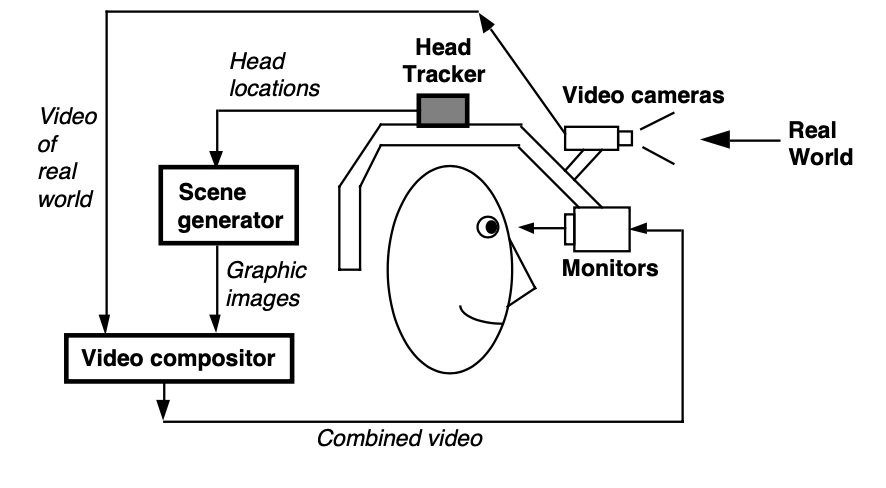
\includegraphics[width=0.75\textwidth]{attachments/Diagram_1.png}
    \caption{Video-Durchsichtiges Display}  \cite{Azuma1997ASO}
    \end{figure}

% On the software side, one of the key tasks is to derive real-world coordinates that are independent of the camera and camera images. This process is known as image registration and involves various computer vision methods, particularly those related to video tracking  \cite{Azuma2001RecentAI}.
Auf der Software-Seite besteht eine der Hauptaufgaben darin, reale Koordinaten abzuleiten, die von der Kamera und den Kamerabildern unabhängig sind. Dieser Prozess wird als Bildregistrierung bezeichnet und umfasst verschiedene Computer-Vision-Methoden, insbesondere solche, die sich auf die Videoverfolgung beziehen \cite{Azuma2001RecentAI}.

    % \newpage


    
\section{Research Methodology}

\subsection{Description of the Benchmark Framework}

\subsubsection{Selection and Categorization of Programming Problems}

Die Entwicklung der Augmented-Reality-Technologie geht auf die 1960er Jahre zurück, als der Informatiker Ivan Sutherland das erste kopfgetragene Display erfand. Dieses bahnbrechende Gerät, das auch als “Sword of Damocles” bezeichnet wurde, ebnete den Weg für tragbare Computerschnittstellen, obwohl es keine echten AR-Funktionen bot \cite{Sutherland1968AHT}. Nicht lange danach, 1975, gründete Myron Krueger den Videoplace, ein Labor für künstliche Realität. Dieser Raum reagierte auf die Bewegungen und Aktionen der Benutzer und machte Brillen oder Handschuhe überflüssig \cite{Videoplace}.

\subsubsection{Characteristics of the Problem Set}

Tatsächlich wurde der Begriff “Augmented Reality” erst 1990 von Thomas P. Caudell, einem ehemaligen Forscher bei Boeing, eingeführt \cite{Lee2012AugmentedRI}. Im Jahr 1992 stellte Louis Rosenburg vom Armstrong Research Lab der United States Air Force “Virtual Fixtures” vor, eines der ersten voll funktionsfähigen Augmented-Reality-Systeme \cite{rosenberg1992use}.

\subsection{Overview of AI Models Evaluated}

Weitere Entwicklungen in den späten 90er Jahren waren die Definition des Realitäts-Virtualitäts-Kontinuums von Paul Milgram und Fumio Kishino im Jahr 1994, das sich von der realen Umgebung zur virtuellen Umgebung erstreckt. Augmented Reality (AR) und Virtual Reality (VR) liegen dazwischen, wobei sich AR zur realen Welt und VR zur virtuellen Welt neigt  \cite{Milgram94a}. Ronald Azumas Studie von 1997 über AR ist ein weiterer wichtiger Meilenstein, der eine allgemein akzeptierte Definition der Technologie liefert. Azuma definierte AR als die Integration von realen und virtuellen Umgebungen mit 3D-Registrierung und Echtzeit-Interaktivität \cite{Azuma1997ASO}. Im Jahr 2000 brachte Hirokazu Kato das AR ToolKit auf den Markt, eine Open-Source-Softwarebibliothek, die die Entwicklung von AR-Softwareanwendungen durch eine Video-Tracking-Technologie revolutionierte, die virtuelle Grafiken über die physische Welt legt \cite{ARTooLKIT}.

\subsection{Evaluation Metrics and Criteria}

In den frühen 2010er Jahren begannen grosse Technologieunternehmen in die AR-Branche einzusteigen. So stellte Google 2012 seine Google Glass vor, eine Augmented-Reality-Brille, die den Nutzern immersive Erfahrungen bietet \cite{Google_for_Developer_2012}. Im Jahr 2015 kündigte Microsoft Windows Holographic und das HoloLens-Headset für Augmented Reality an. Das Headset verschmolz hochauflösende “Hologramme” mit der physischen Welt \cite{Tech_Discussion_2015}. Im Jahr 2016 wurde die Technologie leichter zugänglich, als Niantic Pokémon Go für iOS und Android veröffentlichte. Die mobile AR-App erfreute sich grosser Beliebtheit und steigerte die Attraktivität von AR-Spielen \cite{Bond_2016}. Darüber hinaus hatte der Aufstieg mobiler AR-Apps einen bemerkenswerten Einfluss auf andere Branchen wie den Einzelhandel. Im Jahr 2017 brachte IKEA seine Augmented-Reality-App IKEA Place auf den Markt, die es den Nutzern ermöglicht, sich vor dem Kauf von Möbeln zu Hause eine Vorschau anzusehen \cite{IKEA_2017}. Im Jahr 2023 schliesslich kündigte Apple das Apple Vision Pro an, ein Augmented-Reality-Headset, das die reale und die digitale Welt “nahtlos” miteinander verschmelzen lässt und den neuesten Fortschritt in der AR-Technologie markiert \cite{Apple}.





    \newpage

    \section{Anwendungsgebiete von AR}

\subsection{Archäologie}

Die Technologie der Augmented Reality (“Erweiterte Realität”, AR) findet in der Archäologie Anwendung, insbesondere im Bereich des erweiterten Tourismus. Sie zielt darauf ab, die Erfahrung des Besuchs historischer Stätten zu verbessern, indem virtuelle Rekonstruktionen über die reale Umgebung gelegt werden. Dies wird durch den Einsatz von Geräten wie Head Mounted Displays (HMDs) oder mobilen Geräten erreicht, die virtuelle Objekte über Live-Videoübertragungen legen. Bemerkenswerte Beispiele für diese Technologie sind “ARCHEOGUIDE” und das Projekt “Cultural Heritage Experiences through Socio personal Interactions and Storytelling”.

Über den virtuellen Tourismus hinaus kann AR auch helfen, archäologische Stätten aus einer phänomenologischen Perspektive zu erkunden. Durch die Überlagerung von geografischen Daten aus einem Geografischen Informationssystem (GIS) mit der realen Welt wird eine verkörperte Erfahrung der Landschaft ermöglicht. Dieses Konzept wird anhand eines Projekts in einer bronzezeitlichen Siedlung in Cornwall, Grossbritannien, demonstriert, bei dem eine massstabsgetreue Rekonstruktion der Rundhäuser der Siedlung mit Hilfe einer Spiele-Engine, GIS-Software, einem AR-Plugin und benutzerdefinierten Skripten über die reale Landschaft gelegt wurde. 
\cite{Archaeology}

\subsection{Übersetzung}

Die Technologie der Augmented Reality (“Erweiterte Realität”, AR) wird in vielen Anwendungen eingesetzt, wobei die Übersetzung eine ihrer Anwendungen ist. Ein Beispiel, mit dem viele Menschen vielleicht vertraut sind, aber nicht wissen, dass dort eine AR-Technologie verwendet wird, ist die Word Lens Mobile App, die von Google übernommen und in Google Translate integriert wurde. Mit dieser App können die Nutzer einfach ihre Smartphone-Kamera auf Texte wie Schilder oder Speisekarten richten und bekommen sofort eine Übersetzung neben dem Originaltext auf dem Bildschirm angezeigt. Damit entfällt die Notwendigkeit, ein Foto zu machen oder den Text manuell in die App einzugeben, was für Reisende und Sprachschüler auf der ganzen Welt, die Sprachen verstehen und mit ihnen interagieren wollen, äusserst praktisch ist. \cite{QuestVisual_2010}

\vspace{1cm}

\begin{figure}[ht!]
    \centering
    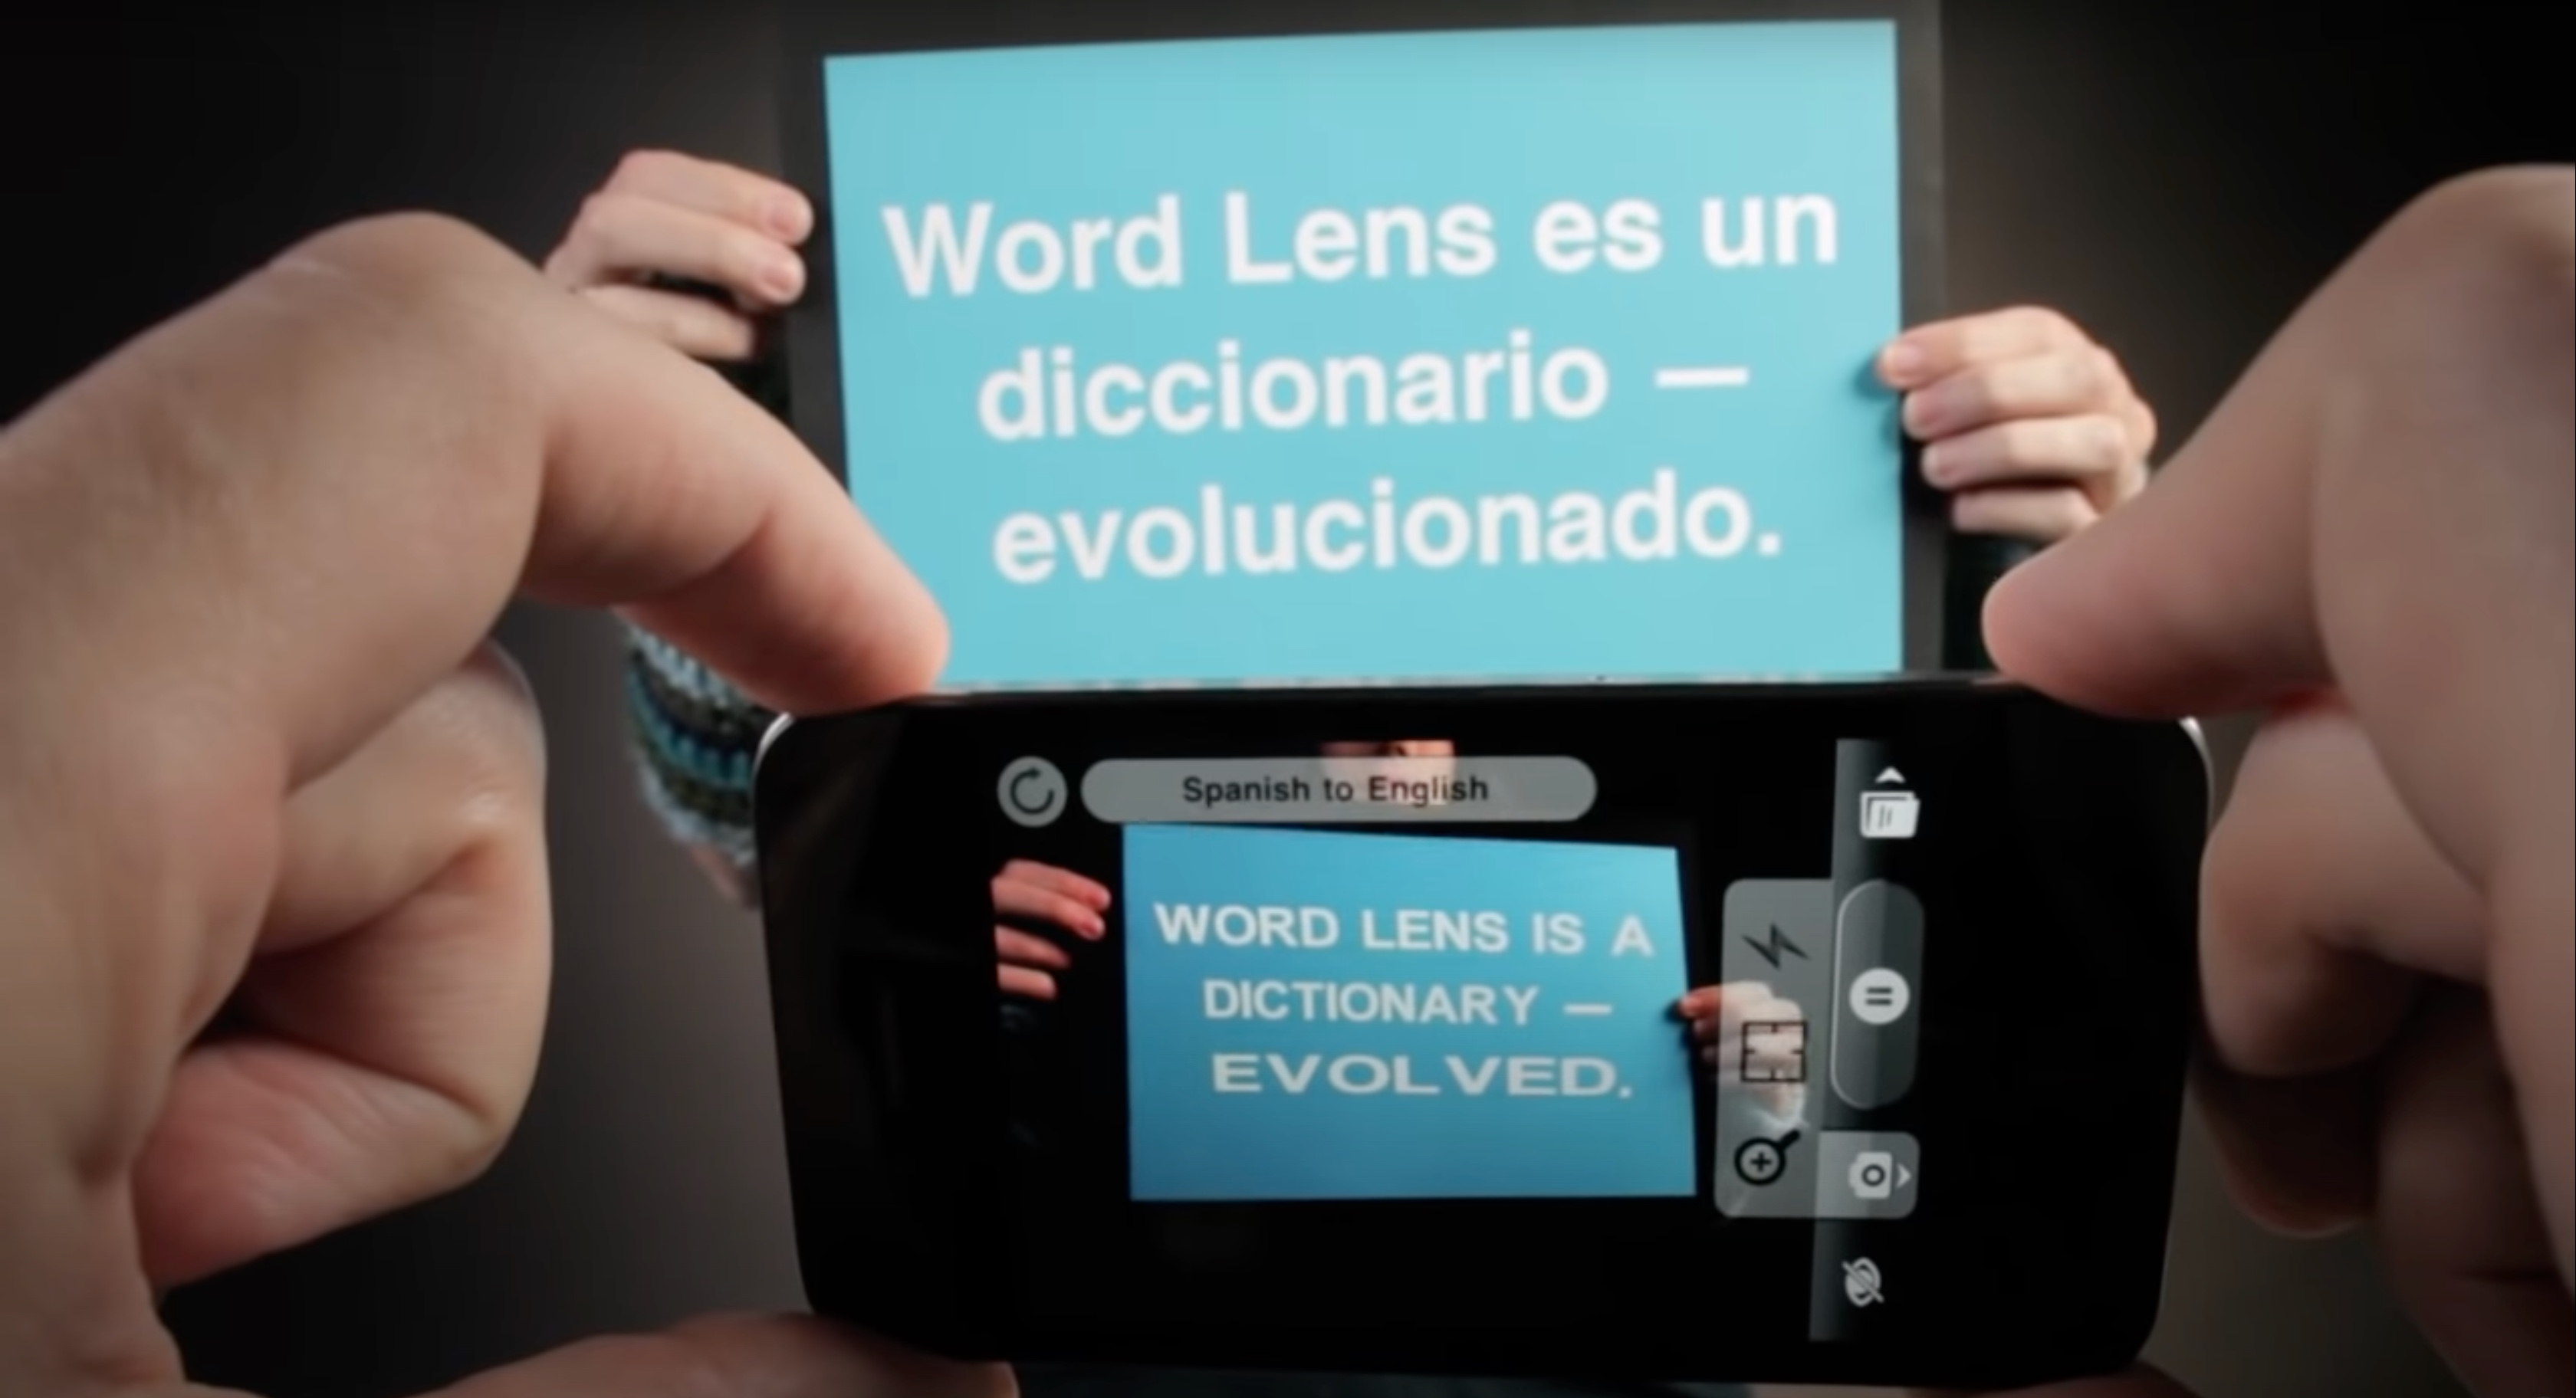
\includegraphics[width=0.7\textwidth]{attachments/Lens.jpeg}
    \caption{Demonstration der Funktionsweise der World Lens} \cite{QuestVisual_2010}
\end{figure}


\subsection{Bildungsbereich}

Augmented Reality (AR) hat das Potenzial, die Bildung durch die Schaffung immersiver Lernumgebungen erheblich zu verändern. Diese Umgebungen ermöglichen es den Lernenden, mit Objekten und Informationen in der realen Welt zu interagieren, was eine praktische und fesselnde Lernerfahrung ermöglicht. AR kann nahtlos in Aktivitäten wie Simulationen, Spiele und Prüfungen integriert werden, um die Entwicklung von kognitiven, emotionalen und physischen Fähigkeiten zu unterstützen. Darüber hinaus bietet AR personalisierte und adaptive Lernerfahrungen, die auf die spezifischen Bedürfnisse der Lernenden zugeschnitten sind und das Interesse, die Motivation und die Zusammenarbeit unter den Schülern fördern. Die pädagogischen Vorteile von AR sind zahlreich, da sie das Behalten von Wissen, die Problemlösungsfähigkeit und die Entscheidungsfindung verbessern und gleichzeitig Kreativität und Innovation fördern. \cite{Wu2013CurrentSO}

Allerdings muss man sich darüber im Klaren sein, dass die Integration von AR in den Unterricht auch mit Herausforderungen verbunden ist. Zu diesen Herausforderungen gehören die Notwendigkeit einer geeigneten Hardware- und Software-Infrastruktur sowie die fehlende Standardisierung verschiedener Plattformen oder Kompatibilitätsprobleme zwischen Systemen oder Geräten. Darüber hinaus besteht die Gefahr, dass die Lernergebnisse beeinträchtigt werden, wenn die Implementierung von AR nicht durchdacht konzipiert oder effektiv durchgeführt wird. Daher müssen Pädagogen und Designer verschiedene Ansätze sorgfältig abwägen und dabei die ethischen Bedenken im Zusammenhang mit dem Einsatz von AR im Bildungsbereich im Auge behalten. Auf diese Weise können sie Strategien und Leitlinien entwickeln, die den Nutzen der erweiterten Realität im Bildungsbereich maximieren.\cite{Wu2013CurrentSO}

\vspace{1cm}

\begin{figure}[h!]
    \centering
    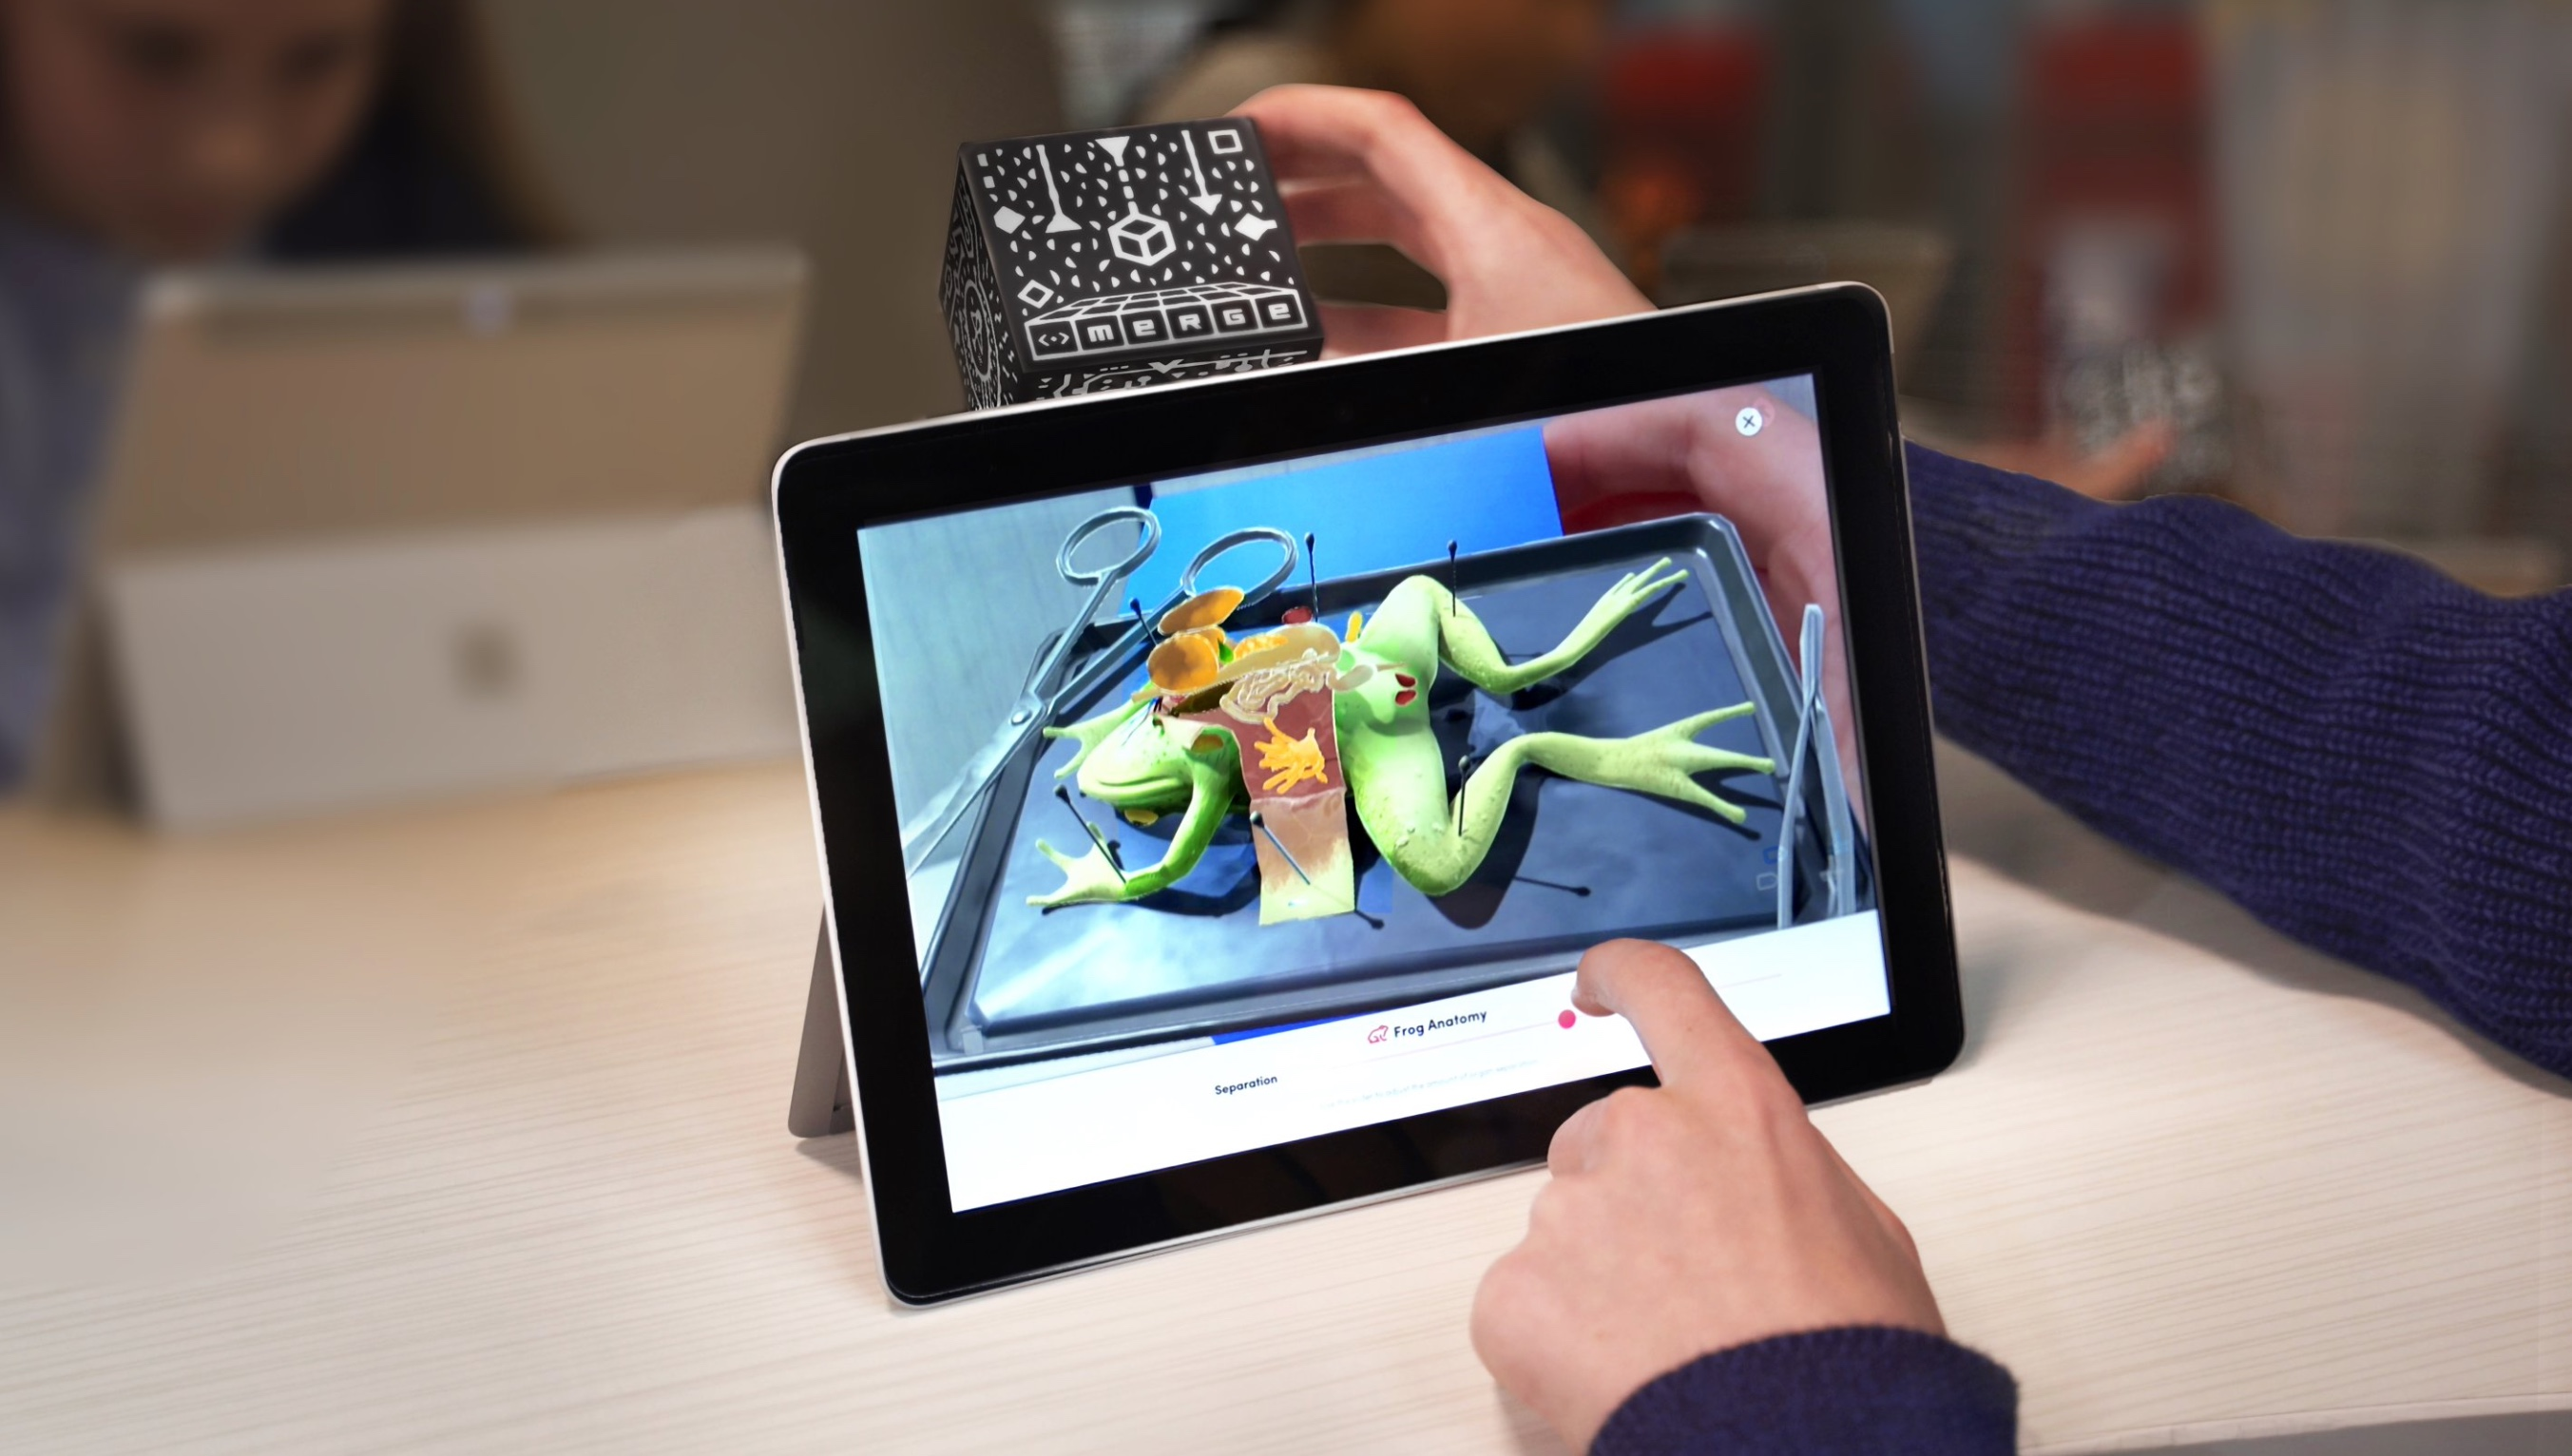
\includegraphics[width=0.7\textwidth]{attachments/cube.jpeg}
    \caption{Schulorientiertes AR-Gerät von Merge EDU} \cite{Merge_EDU}
\end{figure}

\subsection{Videospiele}

Einer der Hauptvorteile der Augmented-Reality-Technologie (AR) in der Videospielindustrie besteht darin, dass sie es den Nutzern ermöglicht, mit synthetischen Objekten, Personen und Umgebungen zu interagieren, die über reale Umgebungen gelegt werden, und ihre Erfahrungen in diesen Umgebungen mit computergenerierten Bildern und Tönen zu erweitern. Dies verbessert das Spielerlebnis und schafft neue Möglichkeiten der sozialen Interaktion. AR-Spiele wie Pokémon GO, Ingress und Zombies, Run! sind bekannte Beispiele für diese Technologie in Aktion. Die körperliche Bewegung, die diese Spiele erfordern, kann jedoch ein Risiko für die Nutzer darstellen, insbesondere wenn sie nicht sicher und verantwortungsvoll genutzt werden. Insgesamt hat AR das Potenzial, die Spieleindustrie zu verbessern und neue und aufregende Erlebnisse für die Spieler zu schaffen. \cite{Das2017AugmentedRV}

\vspace{1cm}

\begin{figure}[ht!]
    \centering
    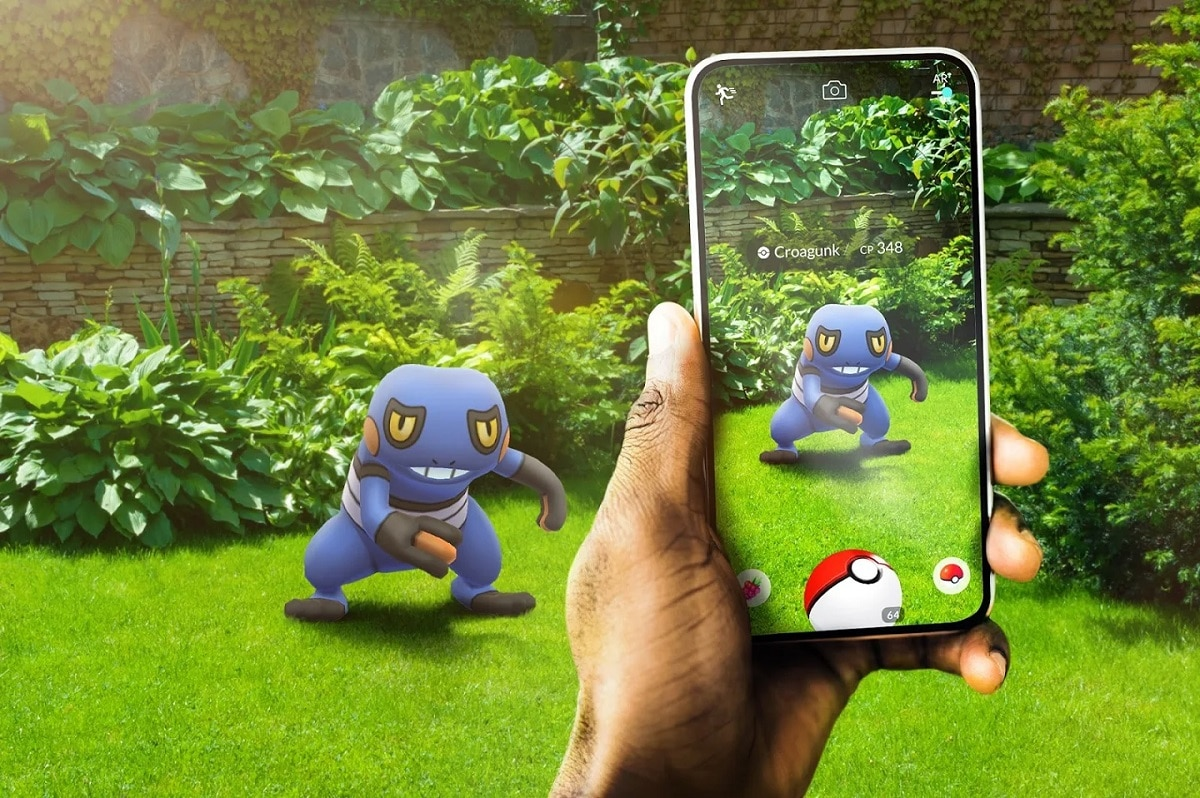
\includegraphics[width=0.7\textwidth]{attachments/pokemon.jpg}
    \caption{AR-Technologie in Pokemon Go verwendet} \cite{Pokemon_GO}
\end{figure}


\subsection{Medizin}
Die Technologie der Augmented Reality (“Erweiterte Realität”, AR) findet in der Praxis Anwendung. Sie ermöglicht die Schaffung von immersiven Lernerfahrungen für Studenten, die komplexe medizinische Konzepte und Verfahren besser verstehen können. \cite{Parsons2021CurrentPO}

Darüber hinaus kann AR Operationen und andere medizinische Verfahren simulieren und so eine kontrollierte Umgebung schaffen, in der die Studenten üben und ihre Fähigkeiten verbessern können. \cite{Parsons2021CurrentPO}

Ausserdem kann Augmented Reality während eines chirurgischen Eingriffs Bilder über den Körper des Patienten legen und dem Chirurgen Anweisungen und Informationen in Echtzeit liefern. Dies trägt dazu bei, die Genauigkeit zu verbessern und Komplikationen bei Operationen zu verringern. \cite{Parsons2021CurrentPO}

AR kann auch eingesetzt werden, um Rehabilitationsprogramme für Patienten zu entwickeln, die sich von Verletzungen oder Operationen erholen. Durch die Bereitstellung von Feedback und Anleitungen werden die Patienten bei der Durchführung von Übungen unterstützt und ihre Fortschritte werden im Laufe der Zeit verfolgt. \cite{cavalcanti2018usability}

Schliesslich spielt Augmented Reality auch eine Rolle bei der Beratung und Unterstützung. Sie ermöglicht es Ärzten, mit Patienten zu interagieren, auch wenn sie räumlich weit voneinander entfernt sind. \cite{Hsieh2018PreliminarySO}

\vspace{1cm}

\begin{figure}[h!]
    \centering
    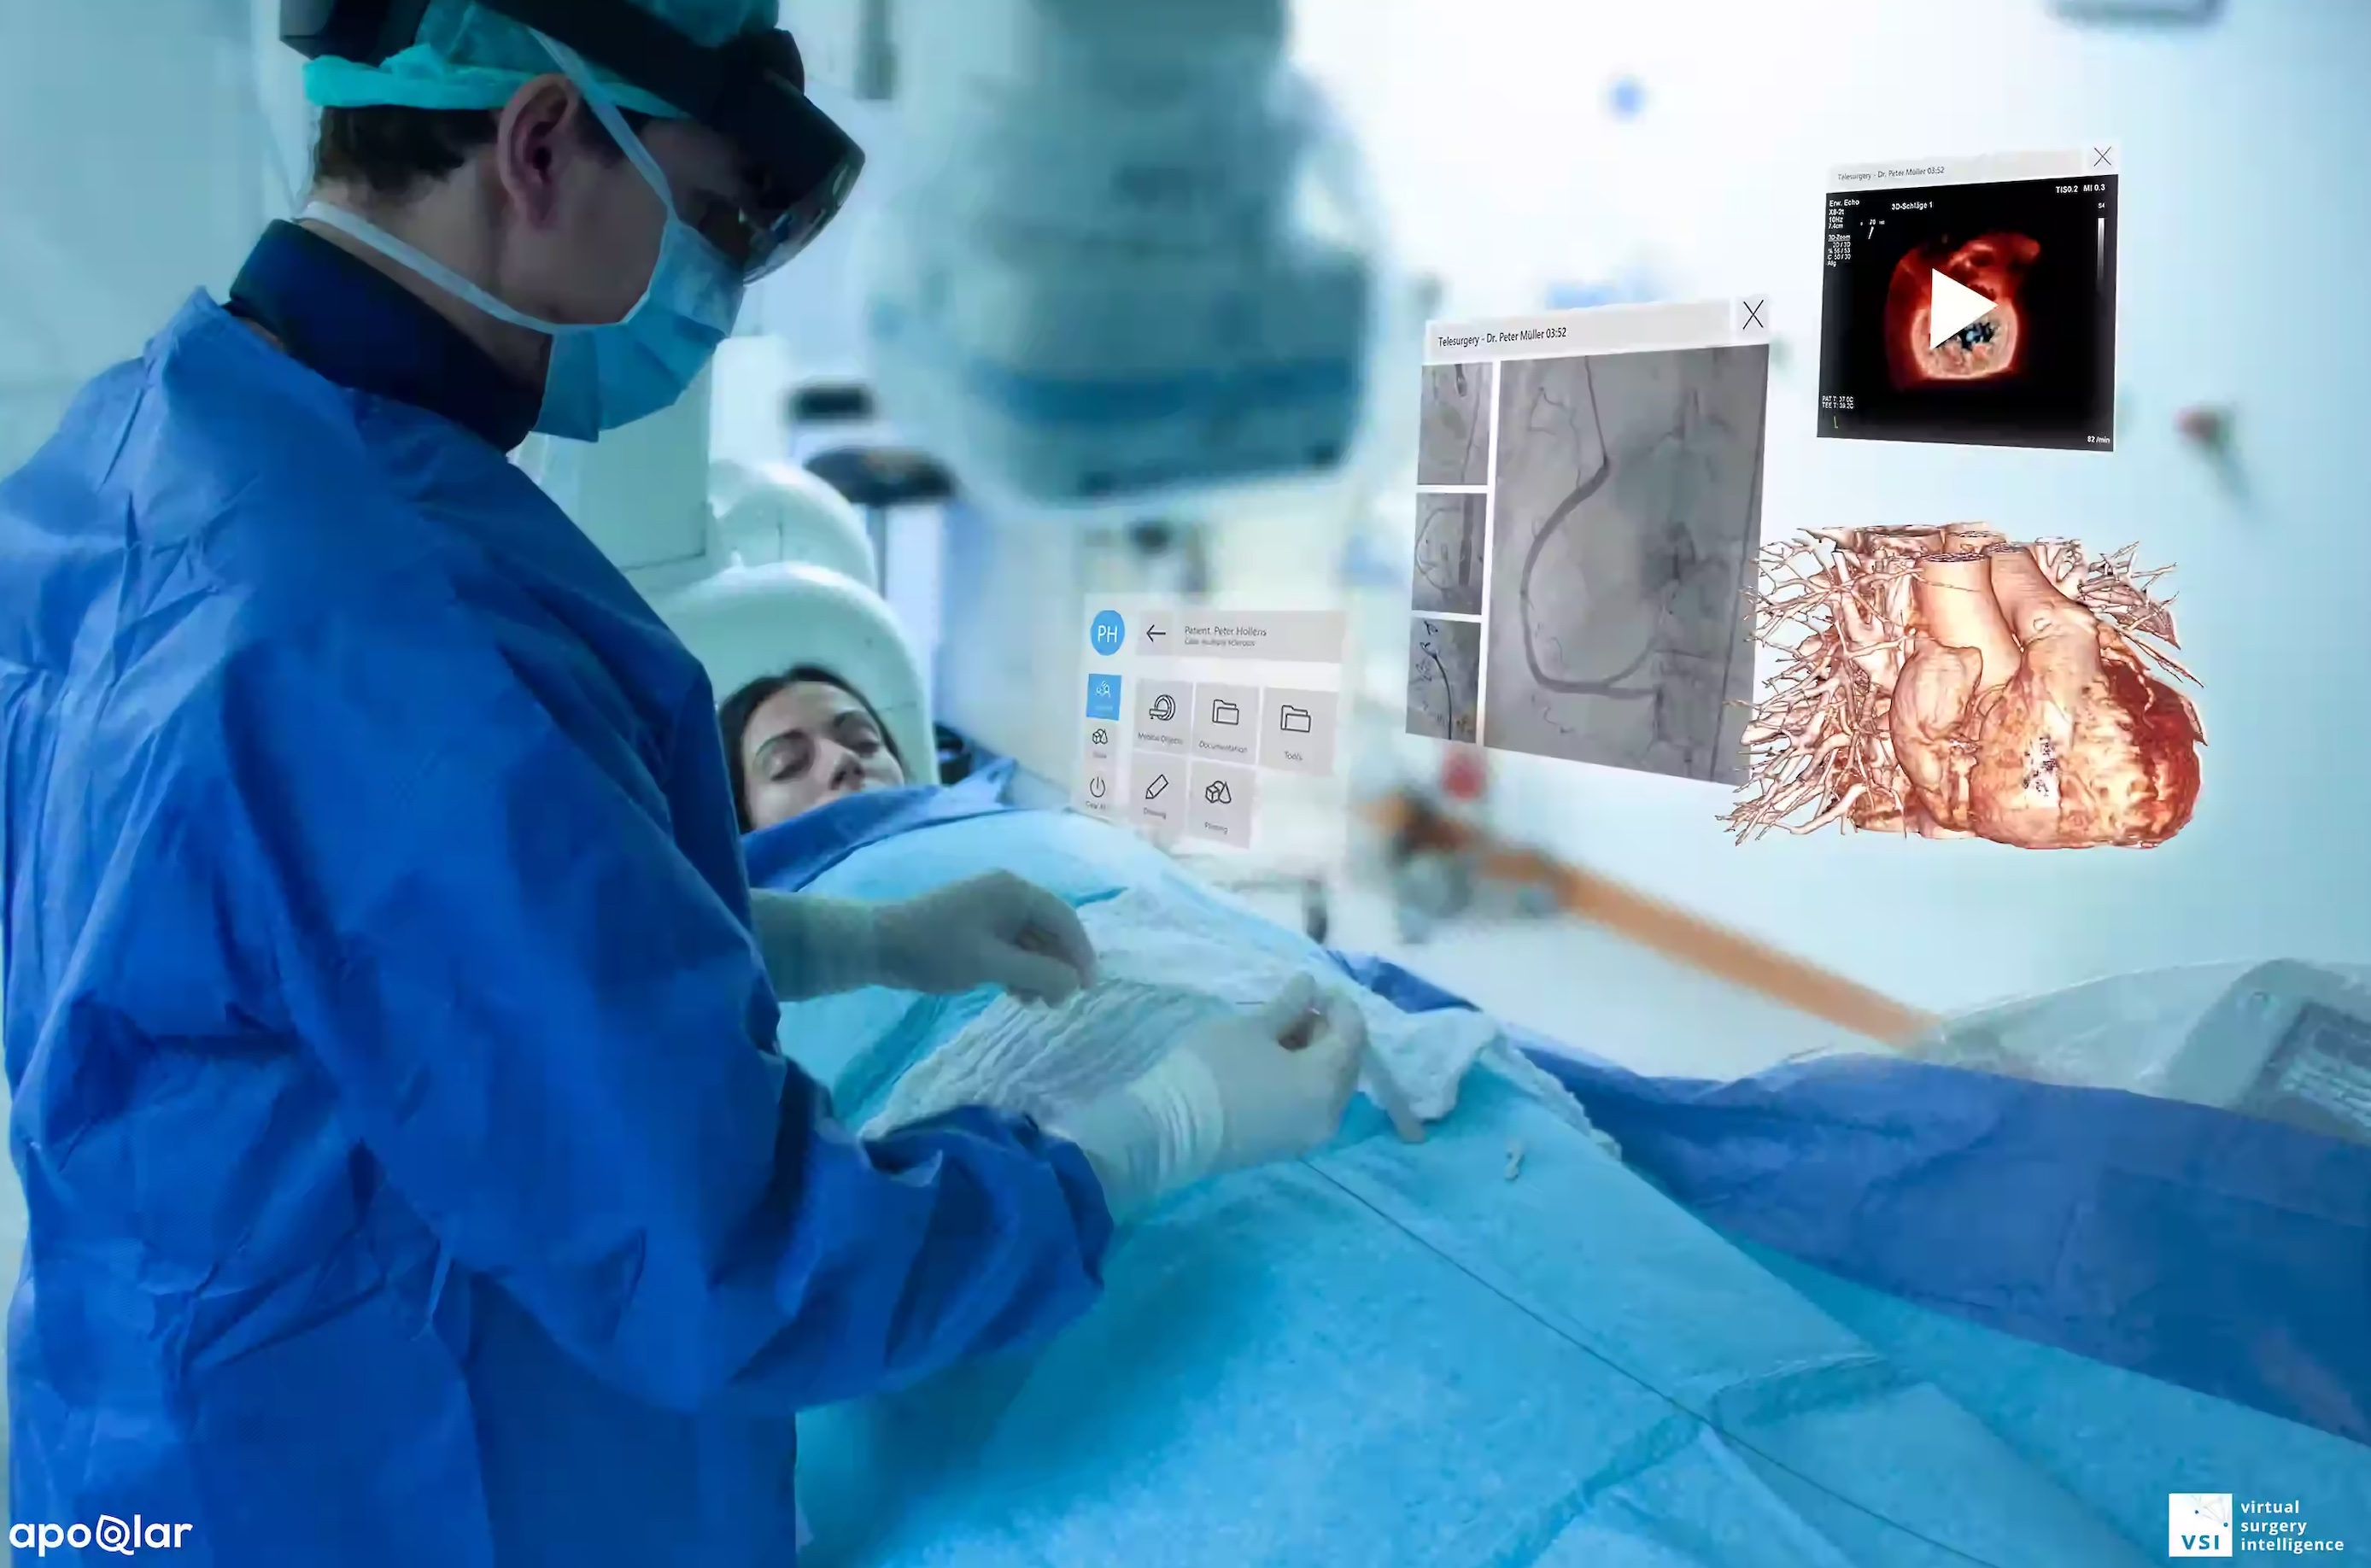
\includegraphics[width=0.7\textwidth]{attachments/surgery.jpeg}
    \caption{Microsoft HoloLens während des Betriebs verwendet} \cite{Microsoft_Healthcare}
\end{figure}

\newpage

\subsection{Militär}
Die AR-Technologie wird auch im Militär eingesetzt, wobei Beispiele aus der realen Welt ihre Wirksamkeit zeigen. Ein Beispiel ist die Nutzung in der Ausbildung, wo sie an der Armeeakademie eingesetzt wurde, um Szenarien zu erstellen, die es Studenten ermöglichen, Trainingssituationen für Bediener zu simulieren und zu modellieren. \cite{Virca2021ApplicationsOA}

Ein weiterer Anwendungsfall ist die Verbesserung des Bewusstseins, wobei Augmented Reality dem Personal Informationen in Echtzeit liefern kann. Diese Echtzeitdaten haben das Potenzial, den gesamten Lebenszyklus militärischer Operationen und die Handlungen des Personals zu begleiten. Darüber hinaus wurden AR-Technologien als kostengünstige Lösung zur Verbesserung der Ausbildung von Soldaten identifiziert. Durch den Einsatz von AR-Technologien können Trainingsprogramme auf die individuellen Bedürfnisse der Soldaten zugeschnitten werden. Darüber hinaus können AR-Technologien computergenerierte Bilder über die Umgebung legen, was die Planung von Operationen erleichtert. \cite{Virca2021ApplicationsOA}

Zusammenfassend lässt sich sagen, dass AR-Technologien die Effizienz von Aktivitäten und Operationen verbessern können, indem sie das Bewusstsein schärfen und dem Personal Informationen in Echtzeit liefern. \cite{Virca2021ApplicationsOA}


\begin{figure}[h!]
    \centering
    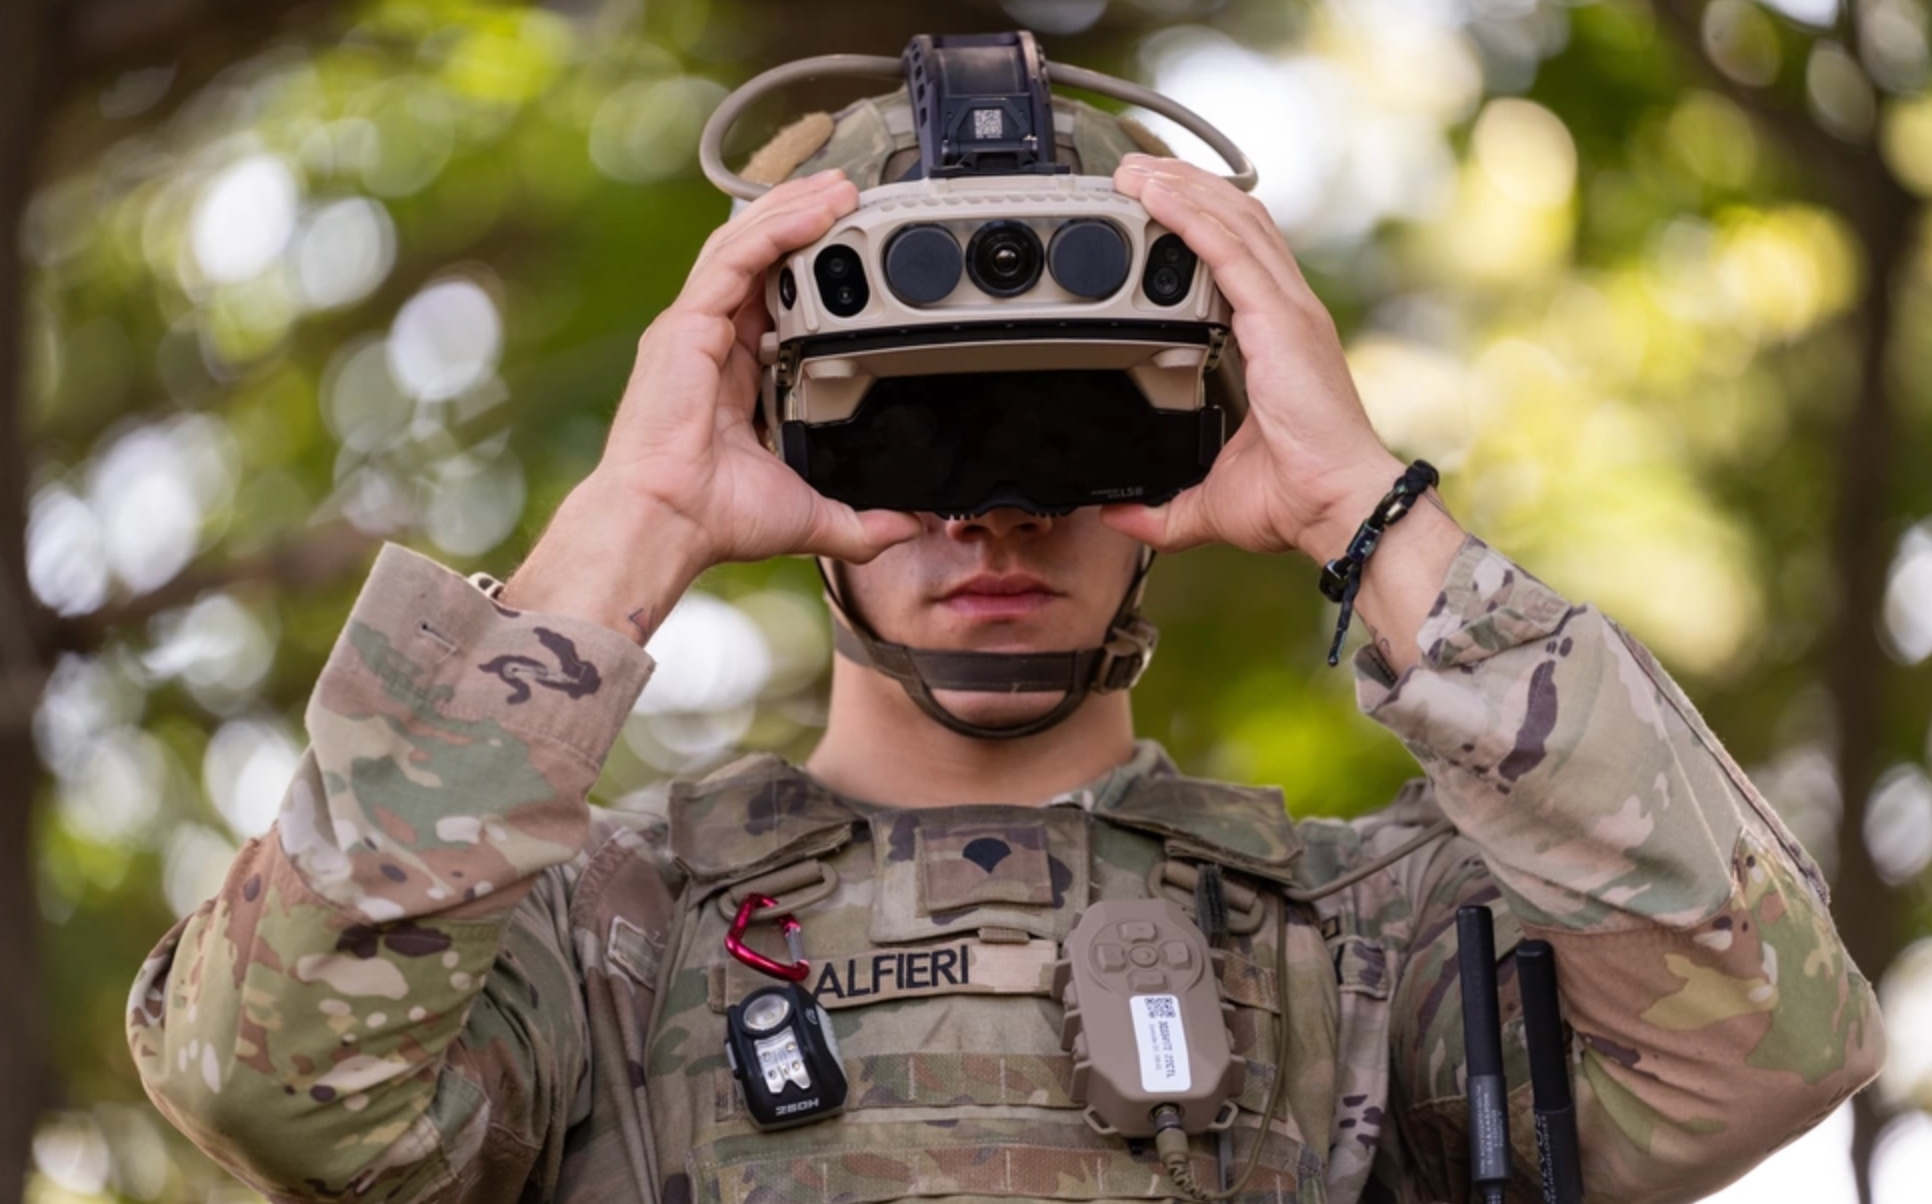
\includegraphics[width=0.5\textwidth]{attachments/army.jpeg}
    \caption{Das Integrated Visual Augmentation (IVAS) System der US-Armee} \cite{Soldier_IVAS}
\end{figure}

\subsection{Navigation}
Wie bereits im geschichtlichen Teil dieses Artikels erwähnt, verwendete das NASA-Raumschiff X-38 ein hybrides System für künstliches Sehen. Dieses System überlagerte Videobilder mit Kartendaten, um die Navigationsfähigkeiten des Raumfahrzeugs zu verbessern. Es basierte auf der Software LandForm, die sich besonders bei schlechten Sichtverhältnissen bewährte. \cite{Delgado2001HybridSS}

Darüber hinaus kann Augmented Reality (AR) zur Verbesserung von Navigationssystemen eingesetzt werden, indem virtuelle Objekte in die reale Welt eingeblendet werden, was zu einer realistischeren und benutzerfreundlicheren Erfahrung führt. AR kann den Nutzern intuitivere und realistischere Navigationsanweisungen geben, z. B. durch Hervorheben von Orientierungspunkten oder Einblenden von Pfeilen in das Sichtfeld des Nutzers. AR kann auch die Sicherheit erhöhen, da der Nutzer seine Aufmerksamkeit nicht mehr von der Strasse ablenken muss. Das Schweizer Unternehmen Way Ray hat beispielsweise holografische AR-Navigationssysteme entwickelt, bei denen holografische optische Elemente verwendet werden, um alle streckenbezogenen Informationen, einschliesslich Wegbeschreibungen, wichtige Mitteilungen und interessante Punkte, direkt in das Sichtfeld des Fahrers und weit vor das Fahrzeug zu projizieren. \cite{WayRay}


\begin{figure}[ht!]
    \centering
    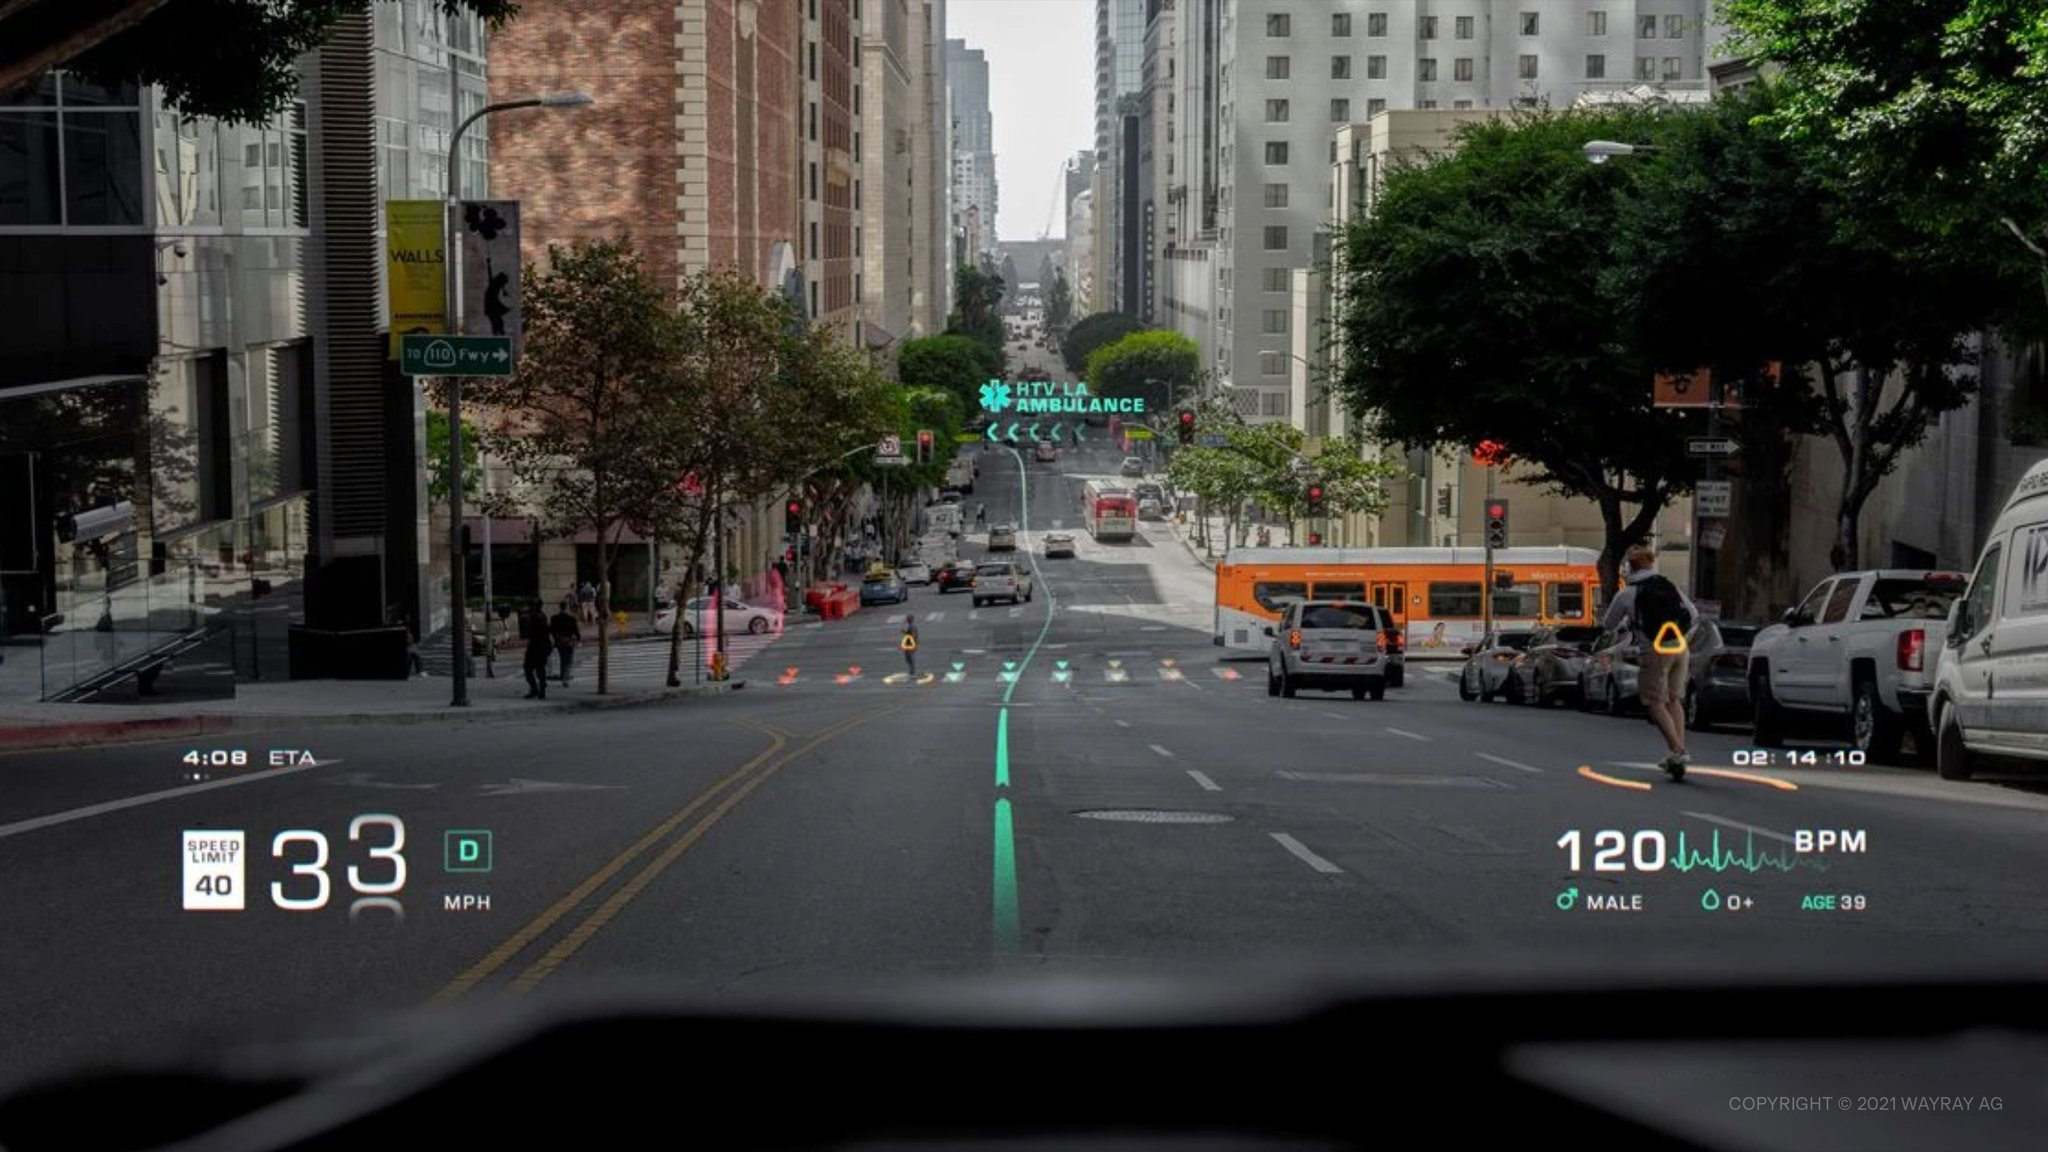
\includegraphics[width=0.6\textwidth]{attachments/wayray.jpg}
    \caption{Das Konzept der in ein Auto integrierten AR-Technologie} \cite{WayRay}
\end{figure}

\subsection{Architektur}
Einer der Vorteile des Einsatzes von AR-Technologie in der Architektur ist die Möglichkeit, dem Nutzer Visualisierungsplattformen für die effektive Verwaltung digitaler Informationen zu bieten. Durch die Integration der AR-Technologie können Architekten Erfahrungen schaffen, die es den Kunden ermöglichen, Entwürfe auf lebensechte Weise zu visualisieren. Dies fördert die Kommunikation zwischen Architekten und Kunden und ermöglicht ein Verständnis des Entwurfs vor Baubeginn. \cite{Chi2013ResearchTA}

Darüber hinaus kann die AR-Technologie auf Baustellen eingesetzt werden, um die Arbeiter bei der Visualisierung von Entwürfen in Räumen zu unterstützen. Dies trägt dazu bei, Fehler zu reduzieren und die Effizienz zu steigern, da die Arbeiter die Platzierung der einzelnen Komponenten genau bestimmen können. Darüber hinaus kann die AR-Technologie Wartungs- und Reparaturanweisungen für Gebäudesysteme bereitstellen, wodurch Ausfallzeiten minimiert und die Sicherheit erhöht werden. \cite{Chi2013ResearchTA}

Ein weiterer Vorteil des Einsatzes von AR-Technologie in der Architektur besteht darin, dass sie den Zugang zu Informationen vor Ort über Dienste ermöglicht. Dies bedeutet, dass Architekten und Bauarbeiter jederzeit und von jedem Ort aus auf projektbezogene Informationen zugreifen können. Eine solche Zugänglichkeit verbessert die Zusammenarbeit zwischen den Teammitgliedern und erleichtert den Arbeitsablauf. \cite{Chi2013ResearchTA}

\subsection{Handel und Marketing}

Augmented Reality wird in der Einzelhandels- und Marketingbranche immer beliebter, um das Kundenerlebnis zu verbessern und die Markentreue zu fördern. Durch den Einsatz von AR können sich die Kunden mit den Produkten auf immersive und personalisierte Weise auseinandersetzen, was zu einer stärkeren Loyalität gegenüber der Marke und höheren Umsätzen führt.

Eine interessante Anwendung der AR-Technologie im Einzelhandel und Marketing ist die Einrichtung von Umkleidekabinen. In diesen virtuellen Räumen können Kunden Kleidung, Accessoires und sogar Make-up anprobieren, ohne in einem Geschäft anwesend zu sein. Unternehmen wie IKEA haben sich diese Technologie zunutze gemacht, um ihren Kunden die Möglichkeit zu geben, sich vor einer Kaufentscheidung ein Bild davon zu machen, wie die Produkte bei ihnen zu Hause aussehen würden. \cite{IKEA_2017}

\vspace{1cm}

\begin{figure}[ht!]
    \centering
    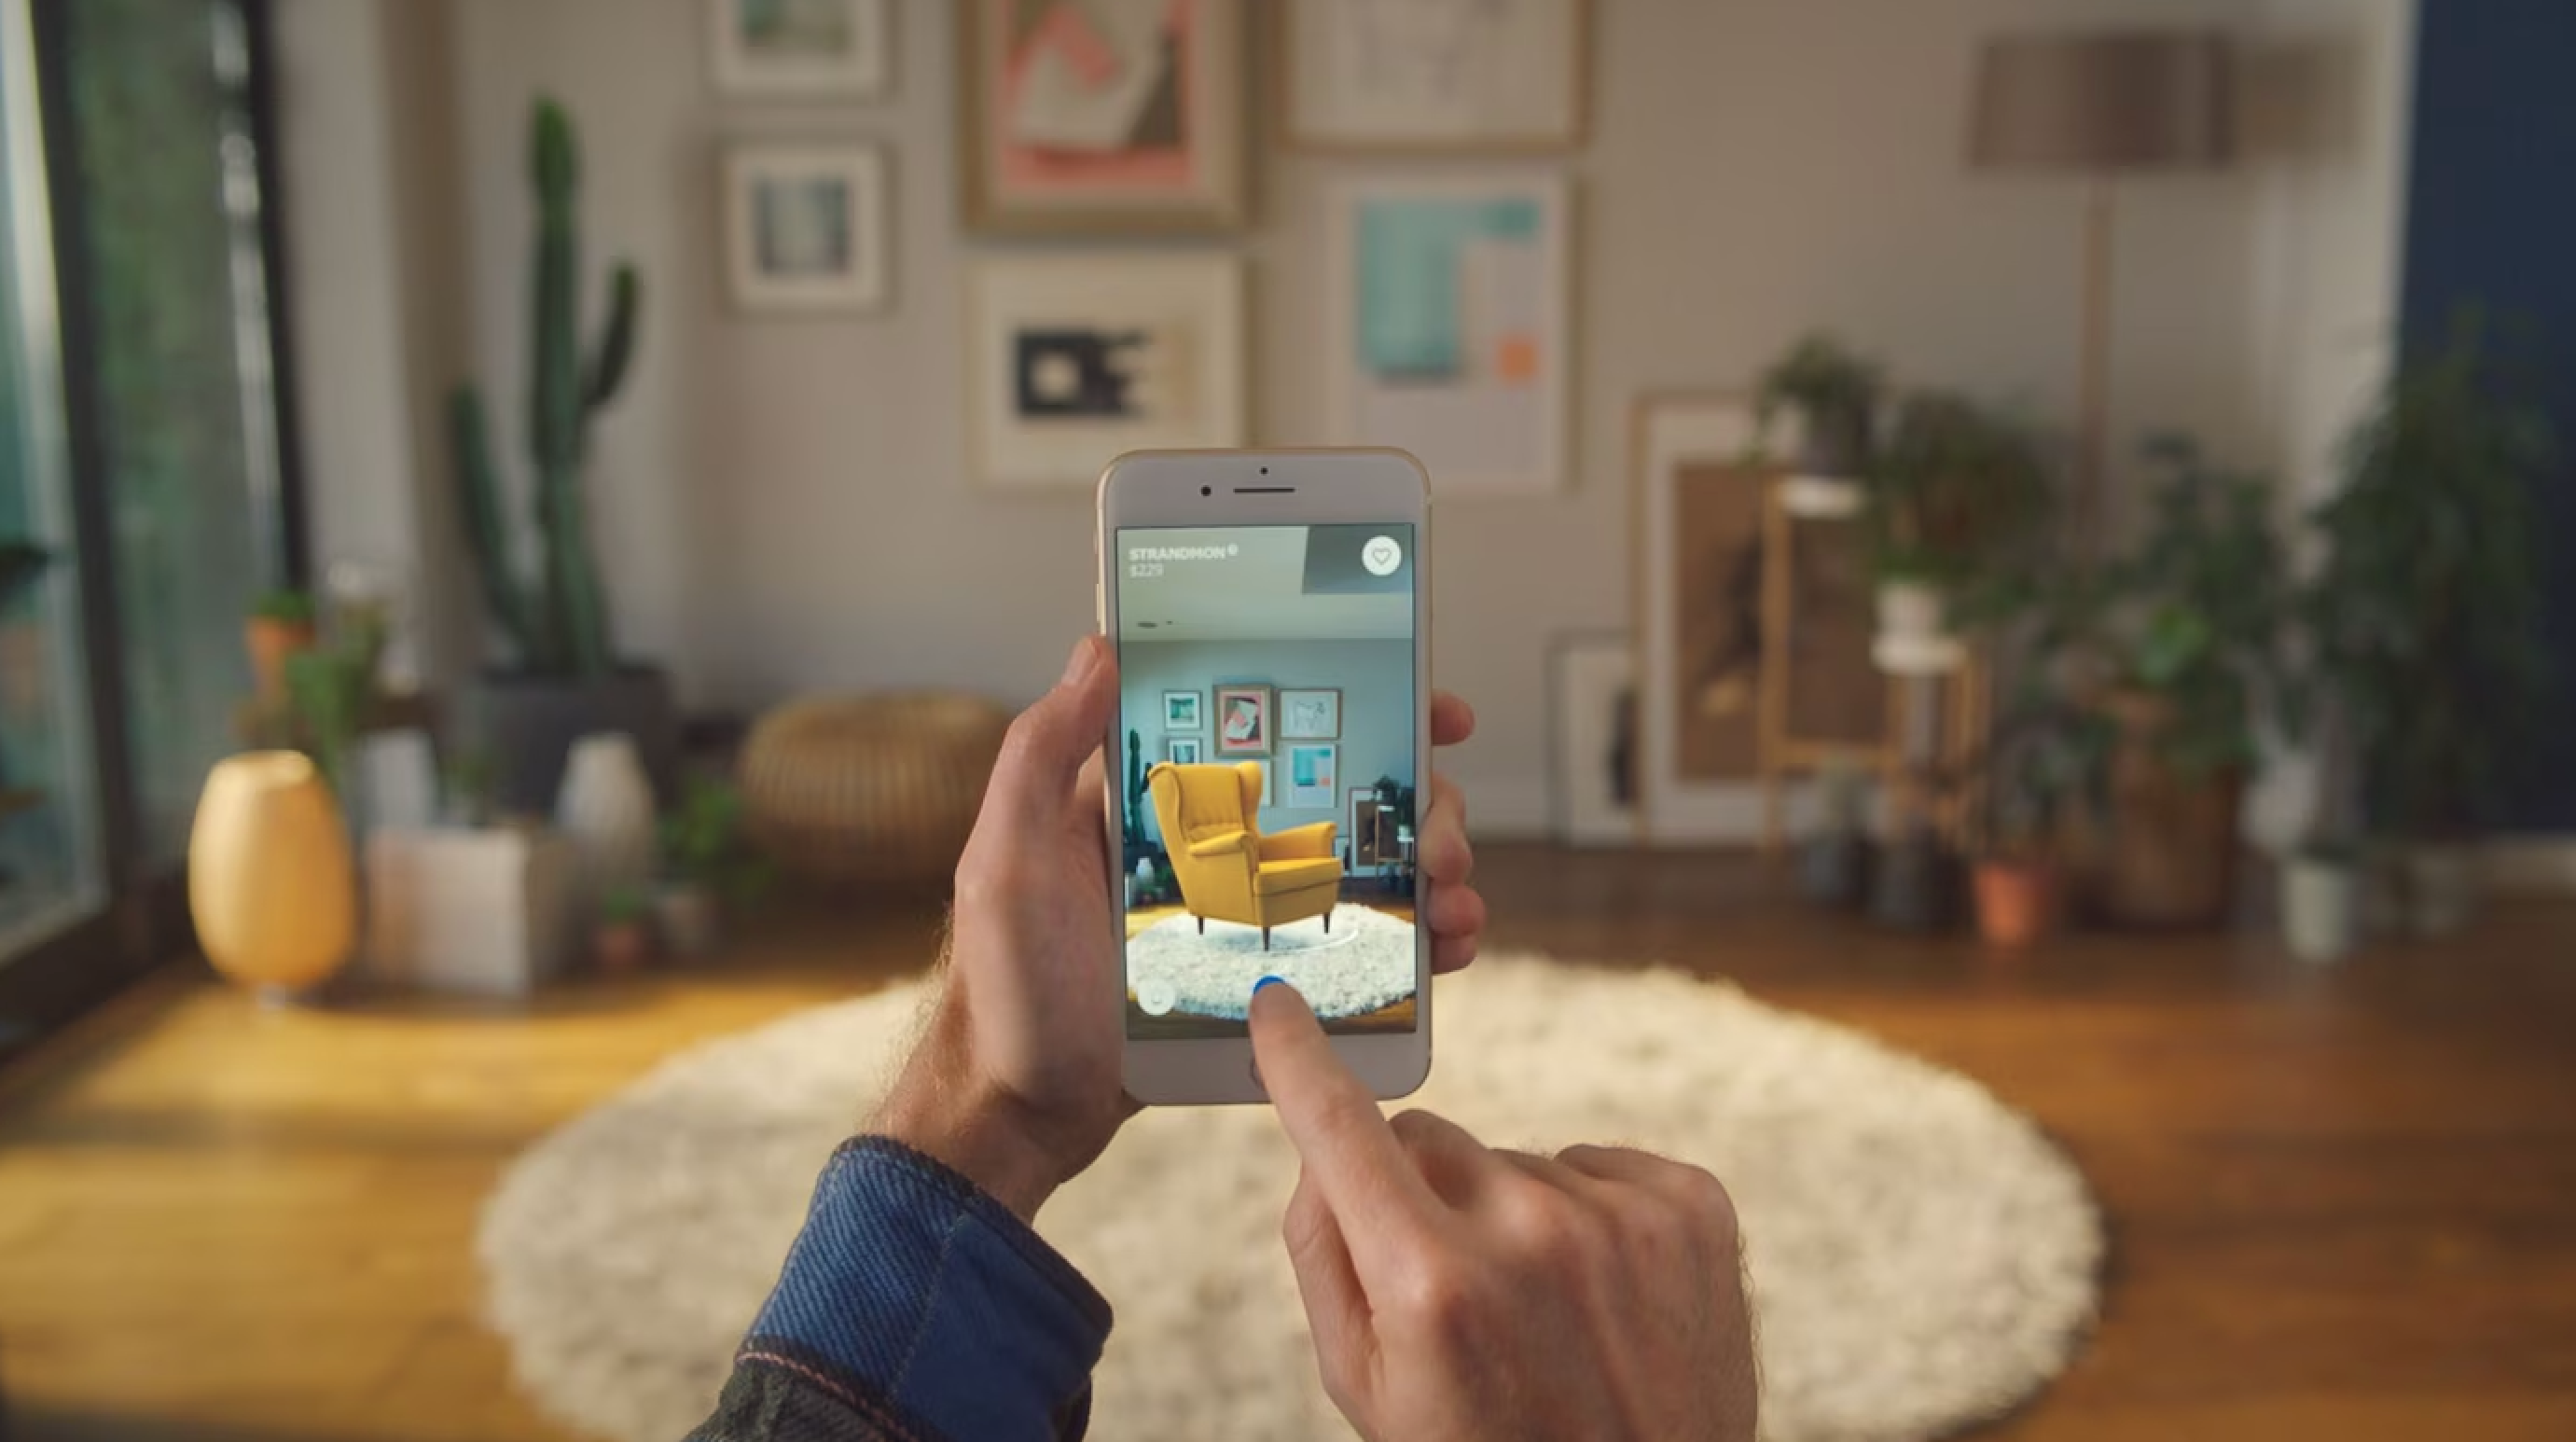
\includegraphics[width=0.6\textwidth]{attachments/ikea.png}
    \caption{IKEA Place im Einsatz} \cite{IKEA_2017}
\end{figure}


Eine weitere Möglichkeit, die AR-Technologie einzusetzen, ist die Visualisierung von Produkten. Sie ermöglicht die Erstellung von 3D-Modellen, mit denen Kunden in einer Umgebung interagieren können. Bekannte Unternehmen wie BMW und Converse nutzen diese Technologie, um ihren Kunden die Möglichkeit zu geben, das Aussehen und die Funktionalität ihrer Produkte in der realen Welt zu erleben \cite{Boeriu_2022}, \cite{Online_Campaigns_2012}

Ausserdem kann die AR-Technologie für standortbezogene Marketingzwecke genutzt werden. Unternehmen haben die Möglichkeit, an bestimmten Orten AR-Erlebnisse zu entwickeln. So könnten sie beispielsweise eine Augmented-Reality-Schnitzeljagd in einem Einkaufszentrum veranstalten oder Informationen über Sehenswürdigkeiten in einer Stadt durch AR bereitstellen.

Zusammenfassend lässt sich sagen, dass die potenziellen Auswirkungen der AR-Technologie auf Handel und Marketing tiefgreifend sind. Indem sie ihren Kunden personalisierte Erlebnisse bieten, können Unternehmen das Engagement erhöhen, die Markentreue fördern und den Umsatz steigern.




    \newpage

    
\section{Results and Analysis}

This section discusses the findings from the benchmark, focusing on quantitative outcomes, comparative analysis of AI model performance, and the insights that emerged from the data.

\subsection{Quantitive Results}

\subsubsection{Success Rates}

Figure 1 illustrates the success rates of the evaluated AI models and the LeetCode baseline among all the problems. There is no suprise that LeetCode solutions achieved the highest success rate, as all the solutions were added programmably. Among the AI models, GPT-3.5 and GPT-4 performed well, with slight differences in handling edge cases and adhering to given templates. Claude and Gemini followed closely, maintaining comparable success rates, showcasing their reliability in solving diverse tasks.

\begin{figure}[H]
    \centering
    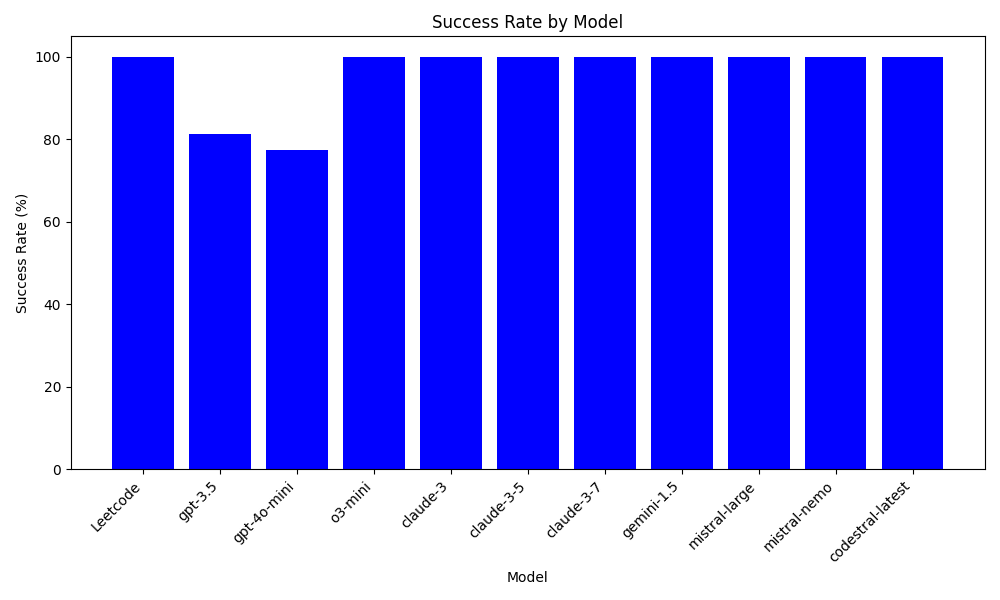
\includegraphics[width=15cm]{attachments/Success_Rate.png}
    \caption{Success Rate by Model} 
\end{figure}



\subsubsection{Runtime Performance}

As shown in Figure 2, LeetCode solutions exhibited the fastest runtime performance, indicating their computational efficiency. In contrast, GPT-4 exhibited slightly slower performance than GPT-3.5, potentially due to its more complex problem-solving mechanisms. Claude and Gemini demonstrated moderate runtime, emphasizing their balanced optimization between speed and accuracy.

\begin{figure}[H]
    \centering
    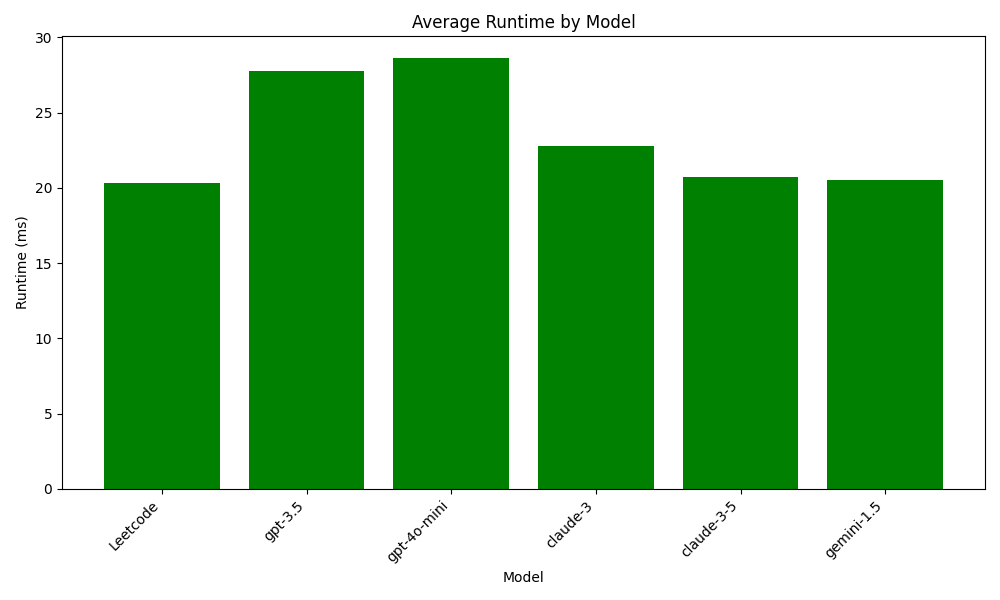
\includegraphics[width=15cm]{attachments/Average_Runtime.png}
    \caption{Average Runtime by Model} 
\end{figure}

\subsubsection{Memory Usage}

Figure 3 highlights the average memory consumption of each model. GPT-3.5 and GPT-4 had the highest memory usage, reflecting their reliance on extensive context processing. Claude and Gemini consumed less memory, showing their efficiency in managing resource utilization. LeetCode solutions required the least memory, indicating their lightweight implementations.

\begin{figure}[H]
    \centering
    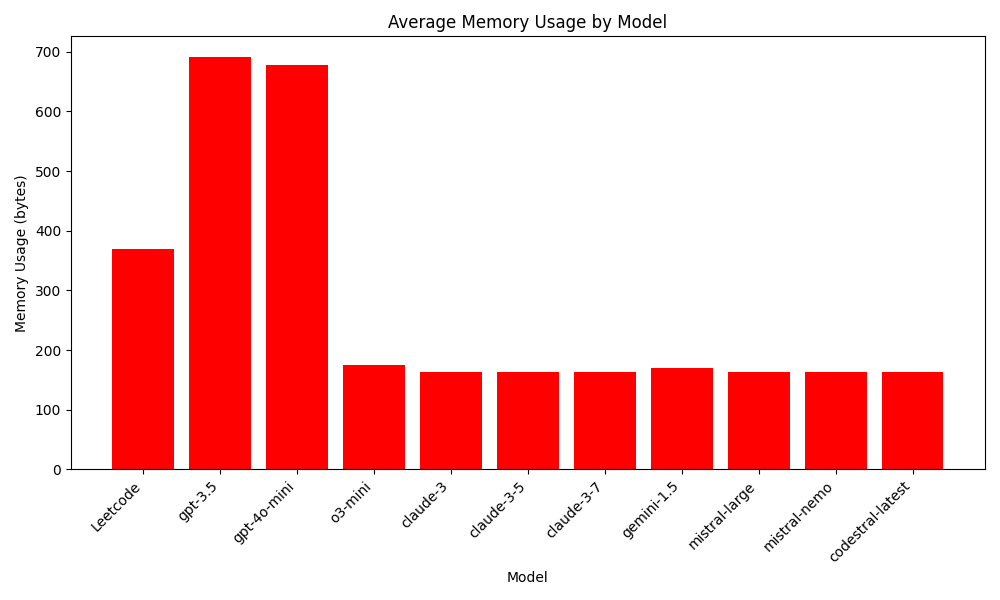
\includegraphics[width=15cm]{attachments/Average_Memory_Usage.png}
    \caption{Average Memory Usage by Model} 
\end{figure}

\subsection{Comparative Performance}

The comparative analysis revealed the trade-offs between speed, accuracy, and memory efficiency across the models. LeetCode solutions set a robust baseline with high accuracy and optimal resource utilization. GPT-3.5 and GPT-4 stood out for their advanced code generation capabilities but required higher computational resources. Claude and Gemini provided competitive performance with slightly lower resource demands, making them suitable for scenarios where memory efficiency is critical.



\subsection{Patterns and Insights}


Several patterns emerged from the analysis. First, the AI models demonstrated consistent success rates across easy and medium problems but showed variability on harder problems, particularly when edge cases or complex logic were involved. This indicates that while AI models excel at standard tasks, they may struggle with unconventional scenarios that require deeper reasoning or specialized knowledge.

Second, runtime and memory usage varied significantly between models. Models like GPT-4, which prioritize contextual understanding, tend to use more memory and exhibit slower runtimes compared to leaner models like Claude. These differences suggest that model selection should align with specific task requirements, balancing efficiency and accuracy.

Overall, the results underscore the growing potential of AI in programming while highlighting areas for improvement. The insights gained from this benchmark provide a foundation for refining AI systems and optimizing their application in real-world software engineering contexts.


















% \section{Implications and Future Directions}

% How AI models can augment current software engineering workflows (e.g., code generation, debugging, and testing).

% Potential changes to roles in the industry (e.g., humans focusing on higher-level tasks while AI handles routine coding).

% Use of AI in education or recruitment (e.g., automated assessment of programming skills).

% \subsection{Implications of Findings for Software Engineering}

% \subsubsection{Selection and Categorization of Programming Problems}

% Impact of problem diversity on AI performance.

% Lessons learned about problem selection and its role in meaningful AI evaluation.

% Recommendations for creating better problem sets in future research.

% \subsubsection{Characteristics of the Problem Set}

% How problem complexity affects AI performance.

% Importance of testing AI models on problems that mirror real-world software engineering challenges.

% The characteristics of the problem set play a crucial role in evaluating the true capabilities of AI models, as the complexity and nature of problems directly influence their performance. The problems used in this study were carefully curated to cover a wide range of scenarios that reflect both theoretical concepts and practical applications in software engineering.

% Problem complexity significantly affects AI performance. Simpler problems, often categorized as "easy," typically involve straightforward logic or basic algorithmic steps, such as iterating through an array or performing simple mathematical calculations. These problems serve as a baseline to assess the AI's ability to produce syntactically and logically correct solutions. AI models generally perform well on these tasks, as they require minimal contextual understanding and rely on commonly observed programming patterns.

% In contrast, more complex problems introduce layers of difficulty that challenge the AI's ability to reason, interpret, and optimize. Medium-difficulty problems often require intermediate skills such as recursion, efficient use of data structures like trees or heaps, or solving problems with moderate constraints. Hard problems push these boundaries further by demanding advanced algorithmic solutions, deep contextual understanding, and the ability to manage multiple interdependent variables. These challenges expose limitations in AI models, such as struggles with abstraction, lack of creativity in designing novel solutions, and inefficiency when faced with computationally intensive tasks.

% The inclusion of problems that mirror real-world software engineering scenarios is crucial for meaningful evaluation. Real-world challenges often involve incomplete or ambiguous problem statements, require multi-step reasoning, or necessitate balancing competing priorities like performance and readability. By incorporating such problems, the study ensures that the evaluation goes beyond textbook scenarios to assess the AI's practical utility. For example, problems that require handling edge cases, implementing scalable solutions, or integrating with existing systems offer valuable insights into the model’s readiness for deployment in professional environments.

% This diverse and thoughtfully constructed problem set enables a comprehensive understanding of the strengths and weaknesses of AI models. It highlights not only their technical capabilities but also their potential limitations when faced with real-world complexity, ultimately guiding future research and development in AI-driven programming tools.
% \subsection{Challenges and Limitations}

% Limitations of the study (e.g., focus on Leetcode, which may not reflect real-world scenarios).

% Challenges in evaluating non-deterministic AI outputs.

% Biases in the dataset or prompts that may influence AI performance.

% \subsection{Future Potential}

% The evolution of AI in software engineering presents a range of opportunities for advancing its role beyond current capabilities. As these models grow more sophisticated, they may achieve a deeper understanding of problem contexts, allowing them to address challenges involving ambiguity or incomplete information with greater precision. By refining their ability to interpret complex requirements, AI systems could become indispensable for tackling tasks that demand both technical knowledge and contextual reasoning.

% In addition to independent problem-solving, AI has the potential to become a more effective collaborator in team-based programming environments. By integrating seamlessly into workflows, these models could assist developers in real time, suggesting optimizations, identifying errors, and improving overall code quality. Such advancements would position AI as a trusted partner in the development process, augmenting rather than replacing human expertise.

% Another promising direction lies in enabling AI to handle large-scale, real-world projects. While current models are adept at solving isolated problems, future systems could extend their functionality to manage multi-file software projects with complex dependencies. This would open doors to applications in fields such as enterprise software development, where AI could assist in creating, maintaining, and scaling systems efficiently.

% The expansion of benchmarks and evaluation frameworks will also play a critical role in shaping the trajectory of AI in programming. By introducing benchmarks that better reflect real-world challenges, such as collaborative tasks or system design problems, researchers can encourage the development of models that align closely with industry needs. This will help bridge the gap between academic research and practical applications, ensuring AI evolves in ways that are directly beneficial to software engineering.

% The ethical implications of relying on AI for critical systems also demand attention. As these systems become more capable, it will be essential to address concerns such as accountability, transparency, and the potential displacement of human roles. By prioritizing responsible development and deployment, AI can be integrated into software engineering in a way that maximizes its benefits while minimizing risks.

% Future advancements in AI for software engineering are likely to reshape the profession in profound ways, enhancing productivity, enabling new possibilities, and driving innovation across the field. As these systems continue to evolve, their role will become increasingly central to the way software is designed, developed, and maintained.








% Suggestions for improving AI models (e.g., better training on real-world coding patterns, handling ambiguities).

% Expanding evaluations to include team-based programming or larger-scale projects.

% Creation of additional benchmarks to assess AI performance in different software engineering tasks (Use my old ideas).



% Do not add the code in Appendix, it is not necessary.


    \newpage

    
\section{Challenges and Adaptations}



\subsection{Encountered Issues}

During the development process, a number of challenges were identified that necessitated adjustments to the initial plan. The primary issues were related to the adaptation of prompt formats, the handling of completely non-functional solutions, and the execution of generated code.
\subsubsection{Generation of Unnecessary Text}
The primary issue that compromised the performance of AI models was the generation of superfluous text. This problem was observed in the GPT-3.5 and GPT-4 models. Despite the imposed limitations in the prompt, the models persistently attempted to generate additional, unnecessary introductory messages. Despite the implementation of enhanced restrictions, GPT models continued to produce code solutions using Markdown syntax, which is employed for inserting code blocks in Markdown files.

\begin{lstlisting}[language=Python]{BitXorMatrix.m}
```python
def twoSum(nums, target):
    num_to_index = {}
    for index, num in enumerate(nums):
        complement = target - num
        if complement in num_to_index:
            return [num_to_index[complement], index]
        num_to_index[num] = index
```
\end{lstlisting}

\subsubsection{Wrong Code Placement}
A further issue that has been identified is the inability of the AI models to generate code that can effectively solve problems in the correct location. Despite the creation of code that could potentially be effective, the AI models disregarded the provided template, for which they were designed to be used.

\begin{lstlisting}[language=Python]{BitXorMatrix.m}
def twoSum(nums, target):
    pass

def two_sum(nums, target):
    num_to_index = {}
    for index, num in enumerate(nums):
        complement = target - num
        if complement in num_to_index:
            return [num_to_index[complement], index]
        num_to_index[num] = index
    \end{lstlisting}

\subsection{Solutions Implemented}

Despite the complexity of these models' behaviour, the solutions to these problems were quite simple in concept.An additional set of restrictions was applied to all the prompts to ensure that no extra text was added to the solution.

The issue with Markdown syntax was resolved by implementing a straightforward function that would verify the first and last lines of the generated code and eliminate any superfluous text.

The misplacement issue was addressed by adding a comment to the template instructing that the code should be written in its place. For illustrative purposes, please refer to the following example:
\begin{lstlisting}[language=Python]{BitXorMatrix.m}
    def twoSum(nums, target):
        # Write your code here
        \end{lstlisting}
    

\subsection{Dropped Approaches}

During the development of the benchmark, several ideas were tested on how to execute the code solutions generated by the AI models. In accordance with the principle of using as few external modules as possible to facilitate easier codebase support in the future, the initial concept was to import each solution as a module. However, the implementation of even the most basic syntax error detection proved to be unnecessarily complicated. Following the decision to measure memory usage as well as runtime, the idea of importing each solution as a module was abandoned. The primary reason for this was that the memory usage of the imported module would be affected by the main process. This would hinder the ability to accurately measure the memory usage of the solution itself. The final approach adopted was to run each solution in a separate sub-process, enabling the memory usage of the solution itself to be measured. This approach also greatly facilitates debugging.















% \section{Implications and Future Directions}

% How AI models can augment current software engineering workflows (e.g., code generation, debugging, and testing).

% Potential changes to roles in the industry (e.g., humans focusing on higher-level tasks while AI handles routine coding).

% Use of AI in education or recruitment (e.g., automated assessment of programming skills).

% \subsection{Implications of Findings for Software Engineering}

% \subsubsection{Selection and Categorization of Programming Problems}

% Impact of problem diversity on AI performance.

% Lessons learned about problem selection and its role in meaningful AI evaluation.

% Recommendations for creating better problem sets in future research.

% \subsubsection{Characteristics of the Problem Set}

% How problem complexity affects AI performance.

% Importance of testing AI models on problems that mirror real-world software engineering challenges.

% The characteristics of the problem set play a crucial role in evaluating the true capabilities of AI models, as the complexity and nature of problems directly influence their performance. The problems used in this study were carefully curated to cover a wide range of scenarios that reflect both theoretical concepts and practical applications in software engineering.

% Problem complexity significantly affects AI performance. Simpler problems, often categorized as "easy," typically involve straightforward logic or basic algorithmic steps, such as iterating through an array or performing simple mathematical calculations. These problems serve as a baseline to assess the AI's ability to produce syntactically and logically correct solutions. AI models generally perform well on these tasks, as they require minimal contextual understanding and rely on commonly observed programming patterns.

% In contrast, more complex problems introduce layers of difficulty that challenge the AI's ability to reason, interpret, and optimize. Medium-difficulty problems often require intermediate skills such as recursion, efficient use of data structures like trees or heaps, or solving problems with moderate constraints. Hard problems push these boundaries further by demanding advanced algorithmic solutions, deep contextual understanding, and the ability to manage multiple interdependent variables. These challenges expose limitations in AI models, such as struggles with abstraction, lack of creativity in designing novel solutions, and inefficiency when faced with computationally intensive tasks.

% The inclusion of problems that mirror real-world software engineering scenarios is crucial for meaningful evaluation. Real-world challenges often involve incomplete or ambiguous problem statements, require multi-step reasoning, or necessitate balancing competing priorities like performance and readability. By incorporating such problems, the study ensures that the evaluation goes beyond textbook scenarios to assess the AI's practical utility. For example, problems that require handling edge cases, implementing scalable solutions, or integrating with existing systems offer valuable insights into the model’s readiness for deployment in professional environments.

% This diverse and thoughtfully constructed problem set enables a comprehensive understanding of the strengths and weaknesses of AI models. It highlights not only their technical capabilities but also their potential limitations when faced with real-world complexity, ultimately guiding future research and development in AI-driven programming tools.
% \subsection{Challenges and Limitations}

% Limitations of the study (e.g., focus on Leetcode, which may not reflect real-world scenarios).

% Challenges in evaluating non-deterministic AI outputs.

% Biases in the dataset or prompts that may influence AI performance.

% \subsection{Future Potential}

% The evolution of AI in software engineering presents a range of opportunities for advancing its role beyond current capabilities. As these models grow more sophisticated, they may achieve a deeper understanding of problem contexts, allowing them to address challenges involving ambiguity or incomplete information with greater precision. By refining their ability to interpret complex requirements, AI systems could become indispensable for tackling tasks that demand both technical knowledge and contextual reasoning.

% In addition to independent problem-solving, AI has the potential to become a more effective collaborator in team-based programming environments. By integrating seamlessly into workflows, these models could assist developers in real time, suggesting optimizations, identifying errors, and improving overall code quality. Such advancements would position AI as a trusted partner in the development process, augmenting rather than replacing human expertise.

% Another promising direction lies in enabling AI to handle large-scale, real-world projects. While current models are adept at solving isolated problems, future systems could extend their functionality to manage multi-file software projects with complex dependencies. This would open doors to applications in fields such as enterprise software development, where AI could assist in creating, maintaining, and scaling systems efficiently.

% The expansion of benchmarks and evaluation frameworks will also play a critical role in shaping the trajectory of AI in programming. By introducing benchmarks that better reflect real-world challenges, such as collaborative tasks or system design problems, researchers can encourage the development of models that align closely with industry needs. This will help bridge the gap between academic research and practical applications, ensuring AI evolves in ways that are directly beneficial to software engineering.

% The ethical implications of relying on AI for critical systems also demand attention. As these systems become more capable, it will be essential to address concerns such as accountability, transparency, and the potential displacement of human roles. By prioritizing responsible development and deployment, AI can be integrated into software engineering in a way that maximizes its benefits while minimizing risks.

% Future advancements in AI for software engineering are likely to reshape the profession in profound ways, enhancing productivity, enabling new possibilities, and driving innovation across the field. As these systems continue to evolve, their role will become increasingly central to the way software is designed, developed, and maintained.








% Suggestions for improving AI models (e.g., better training on real-world coding patterns, handling ambiguities).

% Expanding evaluations to include team-based programming or larger-scale projects.

% Creation of additional benchmarks to assess AI performance in different software engineering tasks (Use my old ideas).



% Do not add the code in Appendix, it is not necessary.

    \newpage

    
\section{Discussion}



\subsection{Capabilities and Limitations of AI Models}

The benchmark showcased AI’s ability to handle algorithmic challenges effectively but highlighted limitations in adaptability and robustness. Models like GPT-4 excelled in generating syntactically correct code but struggled with edge cases and template adherence.


\subsection{Implications for Software Engineering}

The results of the benchmark showed an almost perfect success rate for all problems and AI models. However, there are still many problems to consider. As mentioned earlier, the fact that all the problems were taken from a popular internet source may have played a crucial role in this research. However, it would be premature to say that these results prove that AI is about to overtake all software development jobs. 

A parallel can be drawn with the real interview process. Can we consider a student who has practised a lot of programming problems to be a suitable candidate for a developer role? This is definitely not an easy question to answer, as the job of a software engineer requires other skills, many of which need to be tested in a more complex way. An example of this would be the ability to not only write correct code, but also to work with other people's code, find and fix bugs in it, and so on. In addition, a developer often has to work with external modules, which requires the ability to analyse their documentation.

Ultimately, the results of this benchmark have only revealed the upper level of the AI model's capabilities, and taking into account its success in this test, the next stage of experimentation can and should be carried out.

\subsection{Limitations of the Benchmark}

The benchmark’s focus on algorithmic problems excludes other critical aspects of software engineering, such as maintainability and scalability. Expanding the scope to include these dimensions would provide a more holistic evaluation.


















% \section{Implications and Future Directions}

% How AI models can augment current software engineering workflows (e.g., code generation, debugging, and testing).

% Potential changes to roles in the industry (e.g., humans focusing on higher-level tasks while AI handles routine coding).

% Use of AI in education or recruitment (e.g., automated assessment of programming skills).

% \subsection{Implications of Findings for Software Engineering}

% \subsubsection{Selection and Categorization of Programming Problems}

% Impact of problem diversity on AI performance.

% Lessons learned about problem selection and its role in meaningful AI evaluation.

% Recommendations for creating better problem sets in future research.

% \subsubsection{Characteristics of the Problem Set}

% How problem complexity affects AI performance.

% Importance of testing AI models on problems that mirror real-world software engineering challenges.

% The characteristics of the problem set play a crucial role in evaluating the true capabilities of AI models, as the complexity and nature of problems directly influence their performance. The problems used in this study were carefully curated to cover a wide range of scenarios that reflect both theoretical concepts and practical applications in software engineering.

% Problem complexity significantly affects AI performance. Simpler problems, often categorized as "easy," typically involve straightforward logic or basic algorithmic steps, such as iterating through an array or performing simple mathematical calculations. These problems serve as a baseline to assess the AI's ability to produce syntactically and logically correct solutions. AI models generally perform well on these tasks, as they require minimal contextual understanding and rely on commonly observed programming patterns.

% In contrast, more complex problems introduce layers of difficulty that challenge the AI's ability to reason, interpret, and optimize. Medium-difficulty problems often require intermediate skills such as recursion, efficient use of data structures like trees or heaps, or solving problems with moderate constraints. Hard problems push these boundaries further by demanding advanced algorithmic solutions, deep contextual understanding, and the ability to manage multiple interdependent variables. These challenges expose limitations in AI models, such as struggles with abstraction, lack of creativity in designing novel solutions, and inefficiency when faced with computationally intensive tasks.

% The inclusion of problems that mirror real-world software engineering scenarios is crucial for meaningful evaluation. Real-world challenges often involve incomplete or ambiguous problem statements, require multi-step reasoning, or necessitate balancing competing priorities like performance and readability. By incorporating such problems, the study ensures that the evaluation goes beyond textbook scenarios to assess the AI's practical utility. For example, problems that require handling edge cases, implementing scalable solutions, or integrating with existing systems offer valuable insights into the model’s readiness for deployment in professional environments.

% This diverse and thoughtfully constructed problem set enables a comprehensive understanding of the strengths and weaknesses of AI models. It highlights not only their technical capabilities but also their potential limitations when faced with real-world complexity, ultimately guiding future research and development in AI-driven programming tools.
% \subsection{Challenges and Limitations}

% Limitations of the study (e.g., focus on Leetcode, which may not reflect real-world scenarios).

% Challenges in evaluating non-deterministic AI outputs.

% Biases in the dataset or prompts that may influence AI performance.

% \subsection{Future Potential}

% The evolution of AI in software engineering presents a range of opportunities for advancing its role beyond current capabilities. As these models grow more sophisticated, they may achieve a deeper understanding of problem contexts, allowing them to address challenges involving ambiguity or incomplete information with greater precision. By refining their ability to interpret complex requirements, AI systems could become indispensable for tackling tasks that demand both technical knowledge and contextual reasoning.

% In addition to independent problem-solving, AI has the potential to become a more effective collaborator in team-based programming environments. By integrating seamlessly into workflows, these models could assist developers in real time, suggesting optimizations, identifying errors, and improving overall code quality. Such advancements would position AI as a trusted partner in the development process, augmenting rather than replacing human expertise.

% Another promising direction lies in enabling AI to handle large-scale, real-world projects. While current models are adept at solving isolated problems, future systems could extend their functionality to manage multi-file software projects with complex dependencies. This would open doors to applications in fields such as enterprise software development, where AI could assist in creating, maintaining, and scaling systems efficiently.

% The expansion of benchmarks and evaluation frameworks will also play a critical role in shaping the trajectory of AI in programming. By introducing benchmarks that better reflect real-world challenges, such as collaborative tasks or system design problems, researchers can encourage the development of models that align closely with industry needs. This will help bridge the gap between academic research and practical applications, ensuring AI evolves in ways that are directly beneficial to software engineering.

% The ethical implications of relying on AI for critical systems also demand attention. As these systems become more capable, it will be essential to address concerns such as accountability, transparency, and the potential displacement of human roles. By prioritizing responsible development and deployment, AI can be integrated into software engineering in a way that maximizes its benefits while minimizing risks.

% Future advancements in AI for software engineering are likely to reshape the profession in profound ways, enhancing productivity, enabling new possibilities, and driving innovation across the field. As these systems continue to evolve, their role will become increasingly central to the way software is designed, developed, and maintained.








% Suggestions for improving AI models (e.g., better training on real-world coding patterns, handling ambiguities).

% Expanding evaluations to include team-based programming or larger-scale projects.

% Creation of additional benchmarks to assess AI performance in different software engineering tasks (Use my old ideas).



% Do not add the code in Appendix, it is not necessary.

    \newpage

    
\section{Future Directions and Implications}


\subsection{Expanding the Benchmark}
Expanding the scope of the benchmark is a crucial step for enhancing its relevance and comprehensiveness. While the current benchmark primarily focuses on solving algorithmic problems, programming in real-world settings encompasses a much broader range of tasks. Introducing debugging problems, for example, could assess an AI’s ability to identify and fix errors in existing code, a skill that is fundamental to professional software development yet remains underexplored in most AI evaluations.

Another area of expansion could involve problems requiring the use of external libraries and APIs. These tasks would evaluate how effectively AI models can understand and incorporate pre-existing tools and frameworks into their solutions. Additionally, optimization problems, where the goal is not merely to find a correct solution but the most efficient one, would push AI models to demonstrate advanced resource management and algorithmic ingenuity. By diversifying the problem set to include such challenges, the benchmark could offer a more realistic and nuanced evaluation of an AI model's capabilities in practical programming scenarios.



\subsection{Evaluating More AI Models}
The dynamic nature of AI development necessitates the continuous inclusion of new models to ensure the benchmark remains relevant. While the current version evaluates prominent models like OpenAI’s GPT-4, Anthropic’s Claude, and Google’s Gemini, future iterations should explore additional emerging models. These might include Meta’s LLAMA, specialized models optimized for specific tasks, and other state-of-the-art frameworks developed by research institutions and industry leaders.

By broadening the pool of AI systems under evaluation, the benchmark would provide richer insights into the strengths and weaknesses of different models. This expansion would help in identifying trends across diverse architectures and uncovering areas where further development is needed. Evaluating a variety of models also ensures the benchmark remains a comprehensive tool for analyzing advancements in AI-driven programming.

\subsection{Improving Metrics metrics and Evaluation}

Refining the evaluation metrics is another essential step in advancing the benchmark’s effectiveness. Automating Big O analysis, for instance, could add a deeper layer of assessment by measuring the computational efficiency and scalability of AI-generated solutions. This metric would provide critical insights into the suitability of solutions for real-world applications that involve large datasets or time-sensitive processes.

Stress testing is another promising area for improvement. By running solutions under extreme conditions, such as edge cases or unusually large inputs, the benchmark could evaluate their robustness and resilience. This form of testing would be particularly valuable for assessing how well solutions handle unexpected scenarios, which is often a key requirement in production environments.

Moreover, extending the benchmark to support multiple programming languages would significantly enhance its scope. Evaluating AI models across different languages and coding paradigms would offer a more holistic view of their adaptability and versatility. As modern software engineering often requires proficiency in diverse languages and frameworks, this enhancement would align the benchmark more closely with real-world programming demands.


\subsection{AI Agents for Software Development}


The emergence of AI agents presents an exciting frontier for the benchmark. Unlike traditional models that generate static solutions, AI agents can dynamically interact with external tools, APIs, and environments to solve problems. For example, an AI agent could conduct web searches to gather additional context, leverage APIs to fetch real-time data, or utilize integrated development environments (IDEs) to execute and debug code interactively.

Testing such agents would require a significant rethinking of the benchmark’s structure. New metrics would need to be developed to evaluate their performance effectively, such as the efficiency of multi-step interactions, the accuracy of context-based problem-solving, and the ability to adapt to dynamic requirements. By exploring these advanced capabilities, the benchmark could help illuminate how AI might transition from static problem-solving to dynamic, context-aware programming assistance, further advancing its role in modern software engineering.
















% \section{Implications and Future Directions}

% How AI models can augment current software engineering workflows (e.g., code generation, debugging, and testing).

% Potential changes to roles in the industry (e.g., humans focusing on higher-level tasks while AI handles routine coding).

% Use of AI in education or recruitment (e.g., automated assessment of programming skills).

% \subsection{Implications of Findings for Software Engineering}

% \subsubsection{Selection and Categorization of Programming Problems}

% Impact of problem diversity on AI performance.

% Lessons learned about problem selection and its role in meaningful AI evaluation.

% Recommendations for creating better problem sets in future research.

% \subsubsection{Characteristics of the Problem Set}

% How problem complexity affects AI performance.

% Importance of testing AI models on problems that mirror real-world software engineering challenges.

% The characteristics of the problem set play a crucial role in evaluating the true capabilities of AI models, as the complexity and nature of problems directly influence their performance. The problems used in this study were carefully curated to cover a wide range of scenarios that reflect both theoretical concepts and practical applications in software engineering.

% Problem complexity significantly affects AI performance. Simpler problems, often categorized as "easy," typically involve straightforward logic or basic algorithmic steps, such as iterating through an array or performing simple mathematical calculations. These problems serve as a baseline to assess the AI's ability to produce syntactically and logically correct solutions. AI models generally perform well on these tasks, as they require minimal contextual understanding and rely on commonly observed programming patterns.

% In contrast, more complex problems introduce layers of difficulty that challenge the AI's ability to reason, interpret, and optimize. Medium-difficulty problems often require intermediate skills such as recursion, efficient use of data structures like trees or heaps, or solving problems with moderate constraints. Hard problems push these boundaries further by demanding advanced algorithmic solutions, deep contextual understanding, and the ability to manage multiple interdependent variables. These challenges expose limitations in AI models, such as struggles with abstraction, lack of creativity in designing novel solutions, and inefficiency when faced with computationally intensive tasks.

% The inclusion of problems that mirror real-world software engineering scenarios is crucial for meaningful evaluation. Real-world challenges often involve incomplete or ambiguous problem statements, require multi-step reasoning, or necessitate balancing competing priorities like performance and readability. By incorporating such problems, the study ensures that the evaluation goes beyond textbook scenarios to assess the AI's practical utility. For example, problems that require handling edge cases, implementing scalable solutions, or integrating with existing systems offer valuable insights into the model’s readiness for deployment in professional environments.

% This diverse and thoughtfully constructed problem set enables a comprehensive understanding of the strengths and weaknesses of AI models. It highlights not only their technical capabilities but also their potential limitations when faced with real-world complexity, ultimately guiding future research and development in AI-driven programming tools.
% \subsection{Challenges and Limitations}

% Limitations of the study (e.g., focus on Leetcode, which may not reflect real-world scenarios).

% Challenges in evaluating non-deterministic AI outputs.

% Biases in the dataset or prompts that may influence AI performance.

% \subsection{Future Potential}

% The evolution of AI in software engineering presents a range of opportunities for advancing its role beyond current capabilities. As these models grow more sophisticated, they may achieve a deeper understanding of problem contexts, allowing them to address challenges involving ambiguity or incomplete information with greater precision. By refining their ability to interpret complex requirements, AI systems could become indispensable for tackling tasks that demand both technical knowledge and contextual reasoning.

% In addition to independent problem-solving, AI has the potential to become a more effective collaborator in team-based programming environments. By integrating seamlessly into workflows, these models could assist developers in real time, suggesting optimizations, identifying errors, and improving overall code quality. Such advancements would position AI as a trusted partner in the development process, augmenting rather than replacing human expertise.

% Another promising direction lies in enabling AI to handle large-scale, real-world projects. While current models are adept at solving isolated problems, future systems could extend their functionality to manage multi-file software projects with complex dependencies. This would open doors to applications in fields such as enterprise software development, where AI could assist in creating, maintaining, and scaling systems efficiently.

% The expansion of benchmarks and evaluation frameworks will also play a critical role in shaping the trajectory of AI in programming. By introducing benchmarks that better reflect real-world challenges, such as collaborative tasks or system design problems, researchers can encourage the development of models that align closely with industry needs. This will help bridge the gap between academic research and practical applications, ensuring AI evolves in ways that are directly beneficial to software engineering.

% The ethical implications of relying on AI for critical systems also demand attention. As these systems become more capable, it will be essential to address concerns such as accountability, transparency, and the potential displacement of human roles. By prioritizing responsible development and deployment, AI can be integrated into software engineering in a way that maximizes its benefits while minimizing risks.

% Future advancements in AI for software engineering are likely to reshape the profession in profound ways, enhancing productivity, enabling new possibilities, and driving innovation across the field. As these systems continue to evolve, their role will become increasingly central to the way software is designed, developed, and maintained.








% Suggestions for improving AI models (e.g., better training on real-world coding patterns, handling ambiguities).

% Expanding evaluations to include team-based programming or larger-scale projects.

% Creation of additional benchmarks to assess AI performance in different software engineering tasks (Use my old ideas).



% Do not add the code in Appendix, it is not necessary.
    % Conclusion
    \newpage

    \section{Conclusion}

This research has explored the evolving capabilities of AI in software development, focusing on benchmarking AI models against programming problems to evaluate their potential to substitute or complement human developers. The findings highlight both the strengths and limitations of AI systems like GPT-3.5, GPT-4, Anthropic’s Claude, and Google’s Gemini. While these models excel at generating syntactically correct and often efficient code, their performance is constrained by challenges such as adherence to given function templates, handling edge cases, and generating solutions that are robust under varying conditions.

The benchmark developed in this study provides a comprehensive framework for evaluating AI performance across a range of problem types and difficulty levels. By incorporating metrics like success rate, runtime, and memory usage, the tool offers a nuanced understanding of AI efficiency and effectiveness. The inclusion of multiple AI models has also underscored the diversity of approaches in this domain, revealing areas where individual systems excel or fall short.

However, the study acknowledges the limitations inherent in both the benchmark and the AI models themselves. While the focus has been on algorithmic problems, real-world programming involves a broader spectrum of tasks, including debugging, integration with external tools, and optimization—areas that remain underexplored in this research. These gaps present exciting opportunities for future enhancements, such as expanding the benchmark to include more complex problem types and evaluating emerging AI systems with advanced capabilities.

The implications of these findings extend beyond academic curiosity. As AI continues to evolve, its integration into software development processes promises to reshape the industry. Developers may increasingly rely on AI not just as a coding assistant but as a partner capable of handling complex and dynamic tasks. At the same time, the limitations observed in this study highlight the importance of human oversight, creativity, and expertise—qualities that remain irreplaceable.

In conclusion, this work contributes to the growing body of knowledge on AI’s role in programming by providing a rigorous and adaptable benchmarking tool. It lays the groundwork for further exploration into AI’s capabilities and limitations, offering a foundation for both academic research and practical advancements in the field. The future of AI in software engineering holds immense promise, and this study represents a step toward understanding and harnessing that potential.


    \newpage

    \topskip0pt
    \vspace*{\fill}
    „Hereby, I declare that I have independently prepared the preceding work. All passages that have been quoted or paraphrased have been marked as such.“
    \begin{flushright}
         Andrii Zhabrovets
    \end{flushright}
    \vspace*{\fill}

    
    % Here we import our bibliography(citations) to the document 
    \newpage

    \clearpage

    \bibliography{content/bibliography}



    \newpage
    \addcontentsline{toc}{section}{\listfigurename} % Fuege Abb.vz zu TOC hinzu
    \listoffigures


\end{document}